\chapter{Additional Figures}
\label{ap:addFig}

\section{Chapter 4}
\subsection{Ozone Prior}
\begin{figure}[ht!]
	\centering
	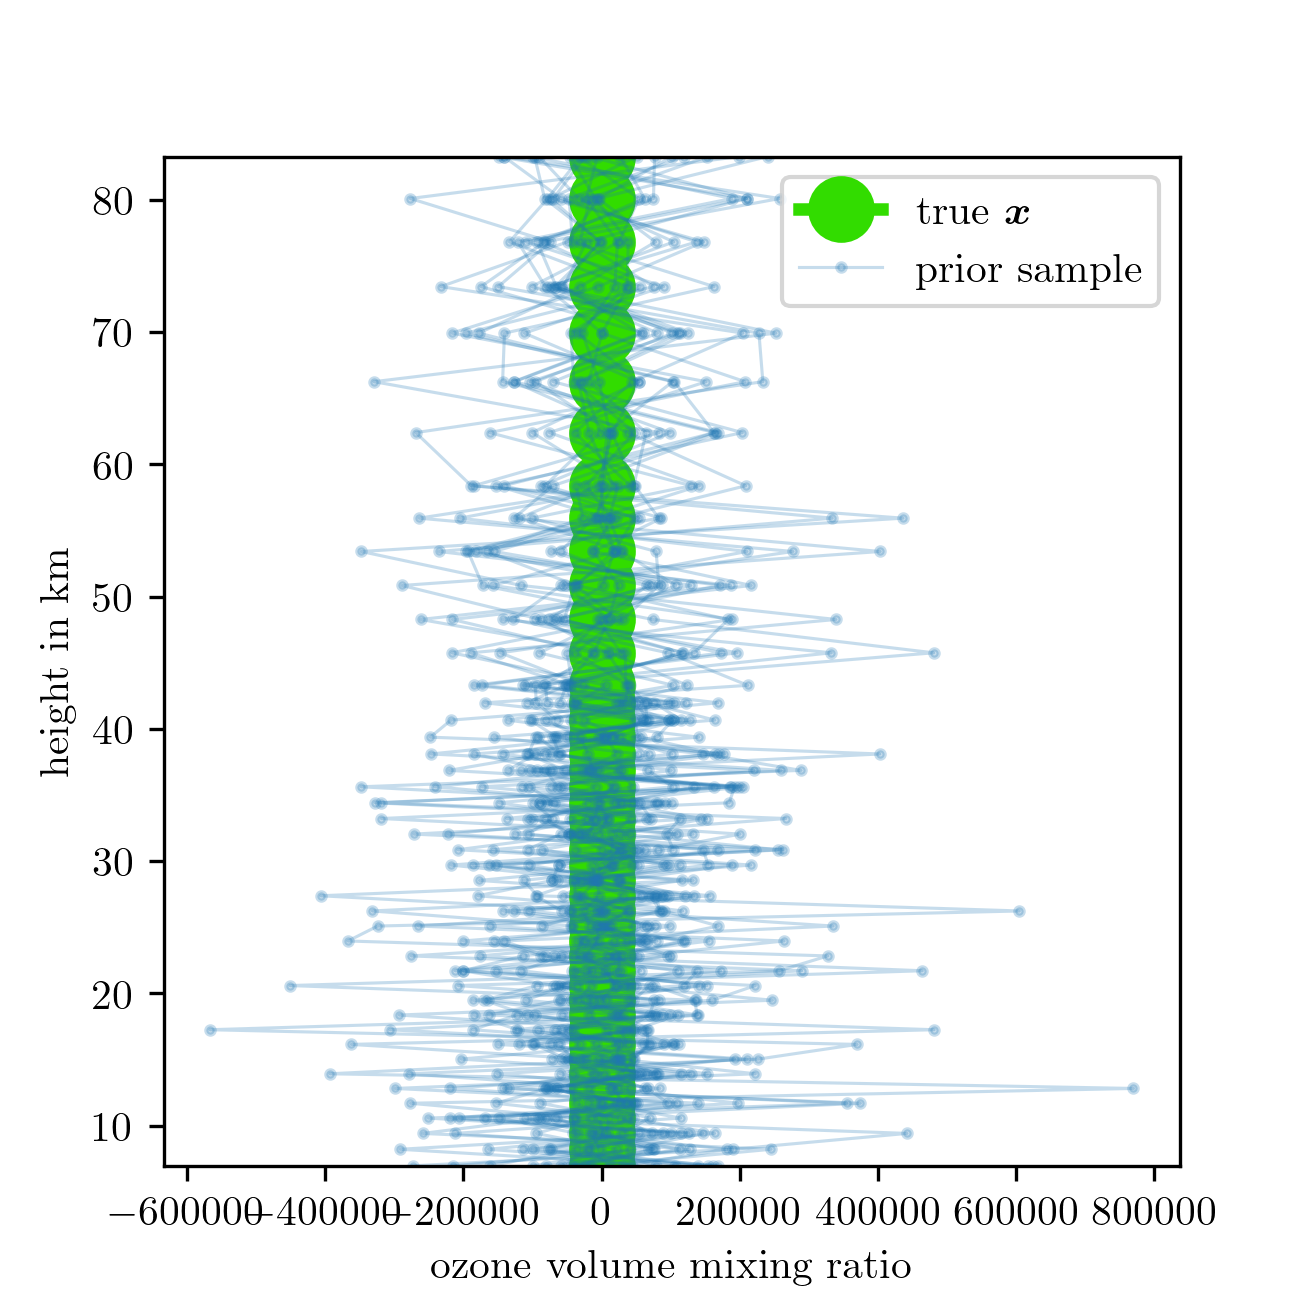
\includegraphics{OzonePrior.png}
	\caption[Samples from ozone prior distribution.]{Prior ozone samples from $\bm{x} \sim \mathcal{N}(0,\delta \bm{L})$ after generating a sample from the hyper-prior distribution $\delta \sim \mathcal{T}(1,10^{-10})$. The true ozone profile appears to be constant due to the variance of prior samples which is not the case, see e.g., Fig.~\ref{fig:O3Samp}.}
	\label{fig:O3Prior}
\end{figure}
\clearpage
\subsection{Integrated Autocorrelation Time} 
\begin{figure}[ht!]
	\centering
	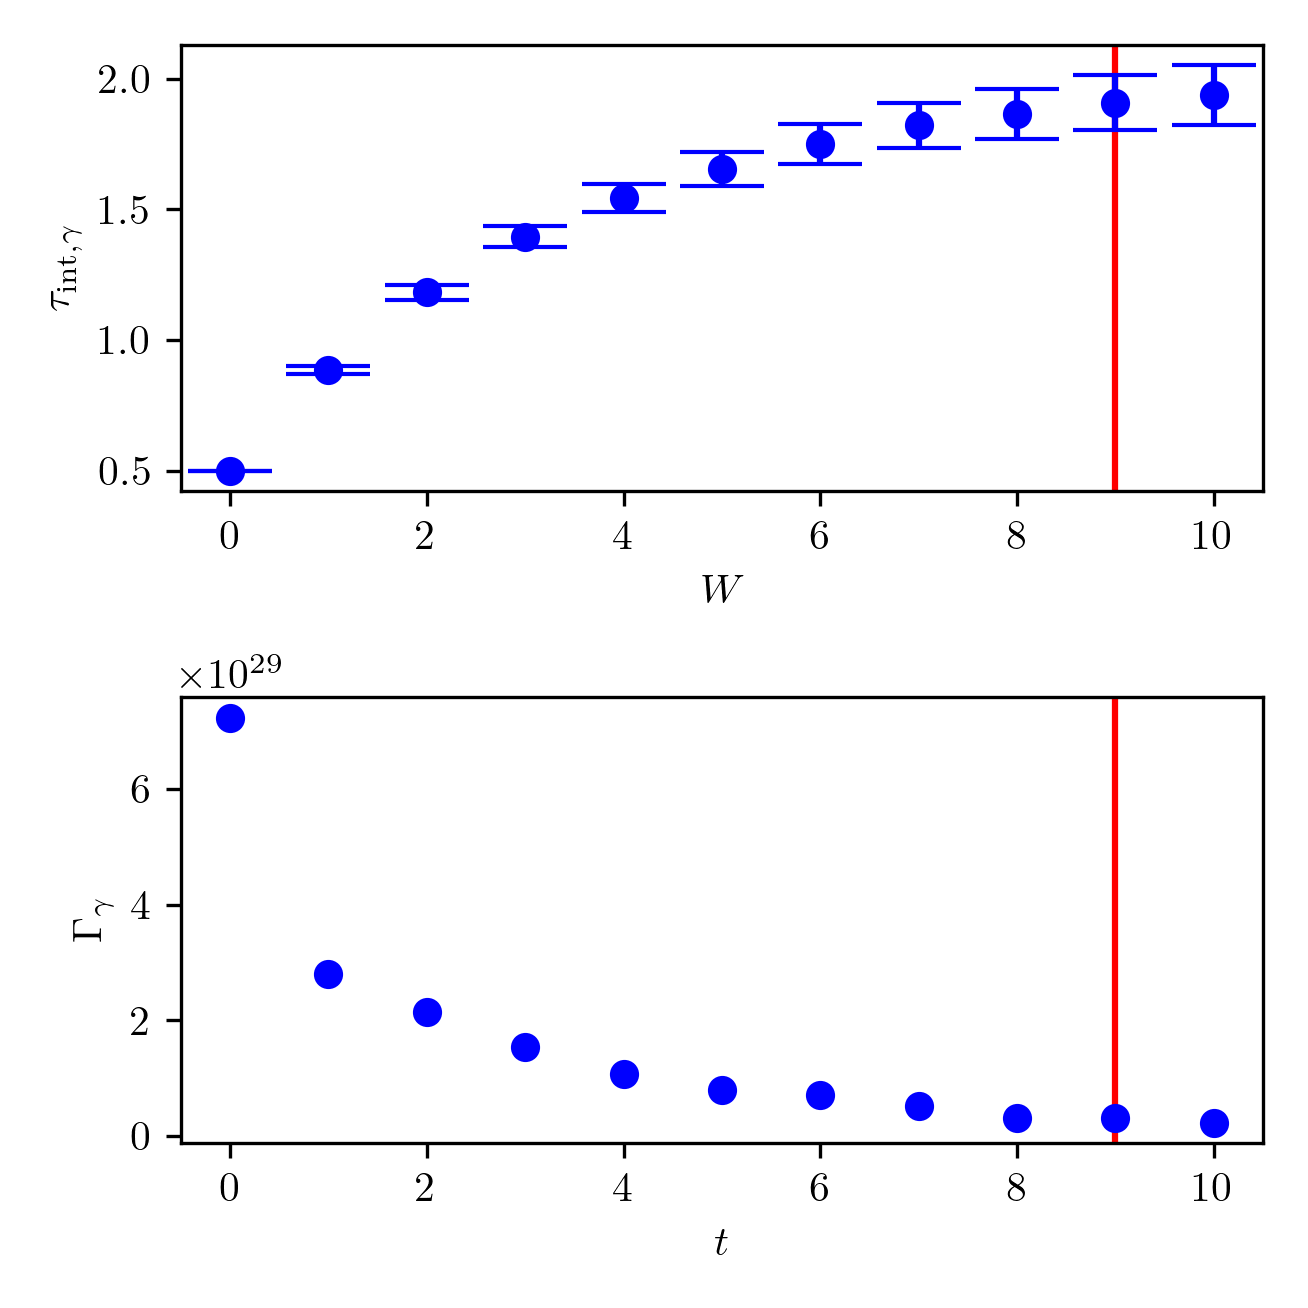
\includegraphics{UwerrTauIntFirstO3gam.png}
	\caption[IACT and autocorrelation of samples $\gamma \sim \pi( \cdot | \bm{y})$, for linear model.]{The IACT $\tau_{\text{int},\gamma}$ at summation windows W as well as the estimated autocorrelation function $\Gamma_{\gamma}$ at lag $t$ of the samples $\gamma \sim \pi(\cdot| \bm{y})$ based on the linear forward model.
	The estimated IACTs are twice the values provided by~\cite{drikHesse, UwerrM}.}
	\label{fig:IATCGamLin}
\end{figure}
\begin{figure}[ht!]
	\centering
	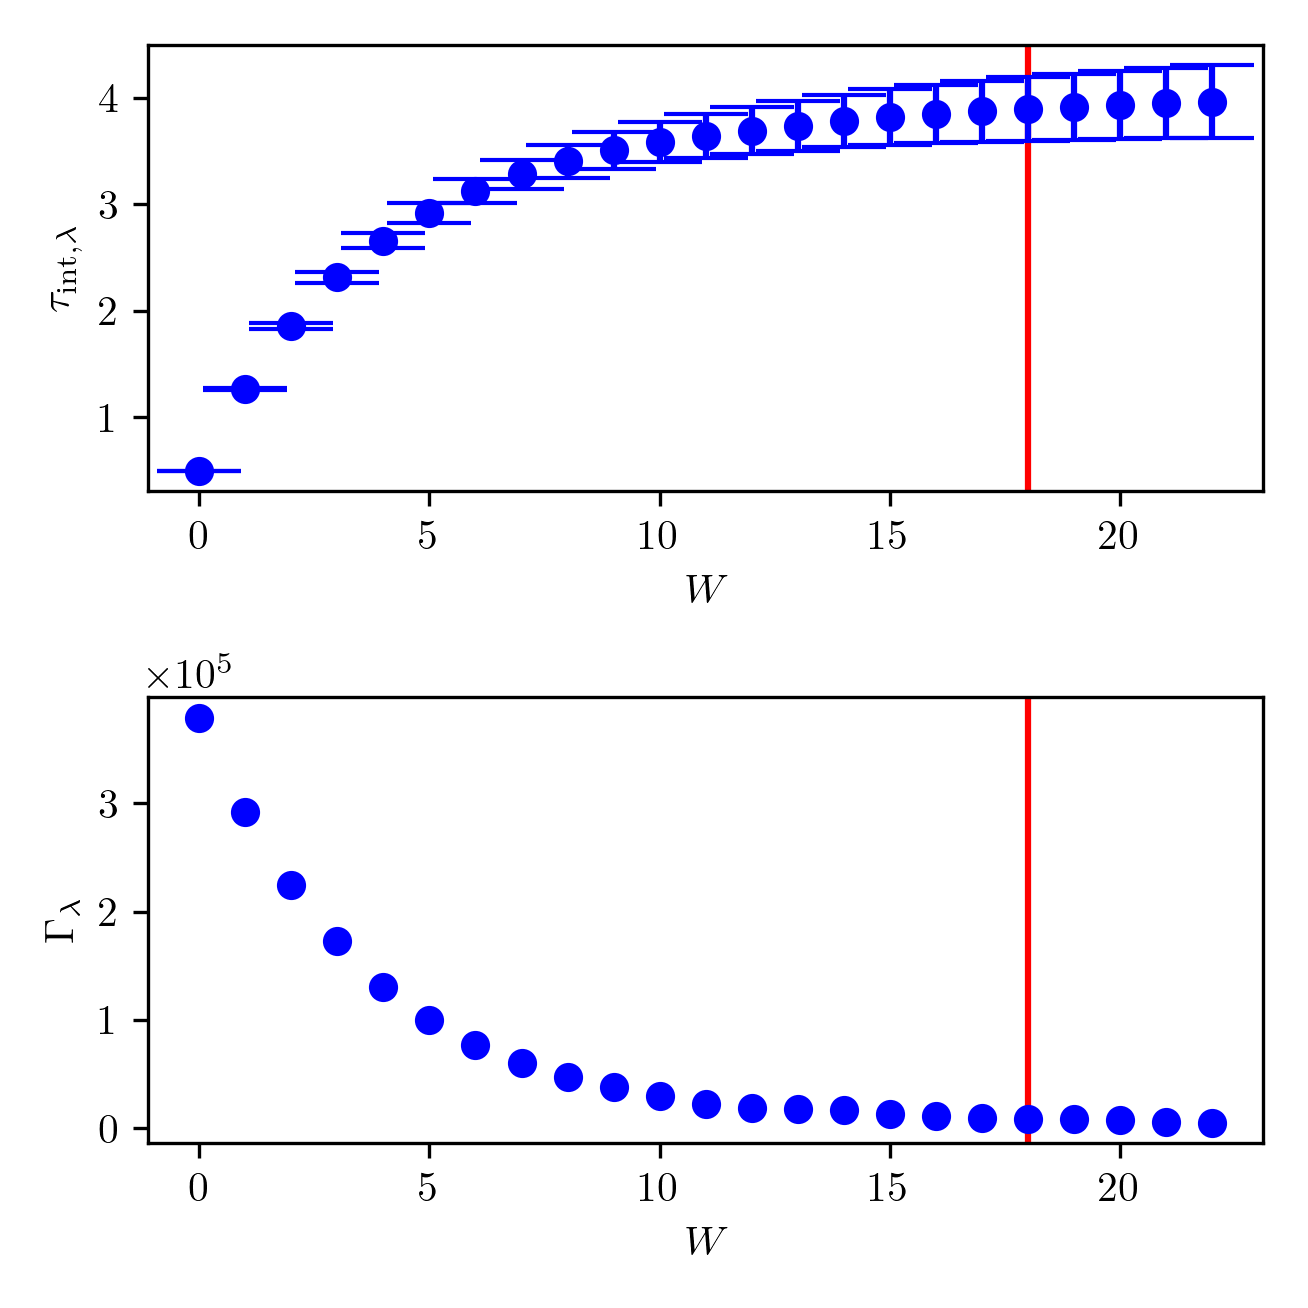
\includegraphics{UwerrTauIntSecO3lam.png}
	\caption[IACT and autocorrelation of samples $\lambda \sim \pi( \cdot | \bm{y})$, for approximated model.]{The IACT $\tau_{\text{int},\lambda}$ at summation windows W as well as the estimated autocorrelation function $\Gamma_{\lambda}$ at lag $t$ of the samples $\lambda \sim \pi( \cdot | \bm{y})$ based on the approximated forward model.
	The estimated IACTs are twice the values provided by~\cite{drikHesse, UwerrM}.}
	\label{fig:IATCSecO3lam}
\end{figure}
\begin{figure}[ht!]
	\centering
	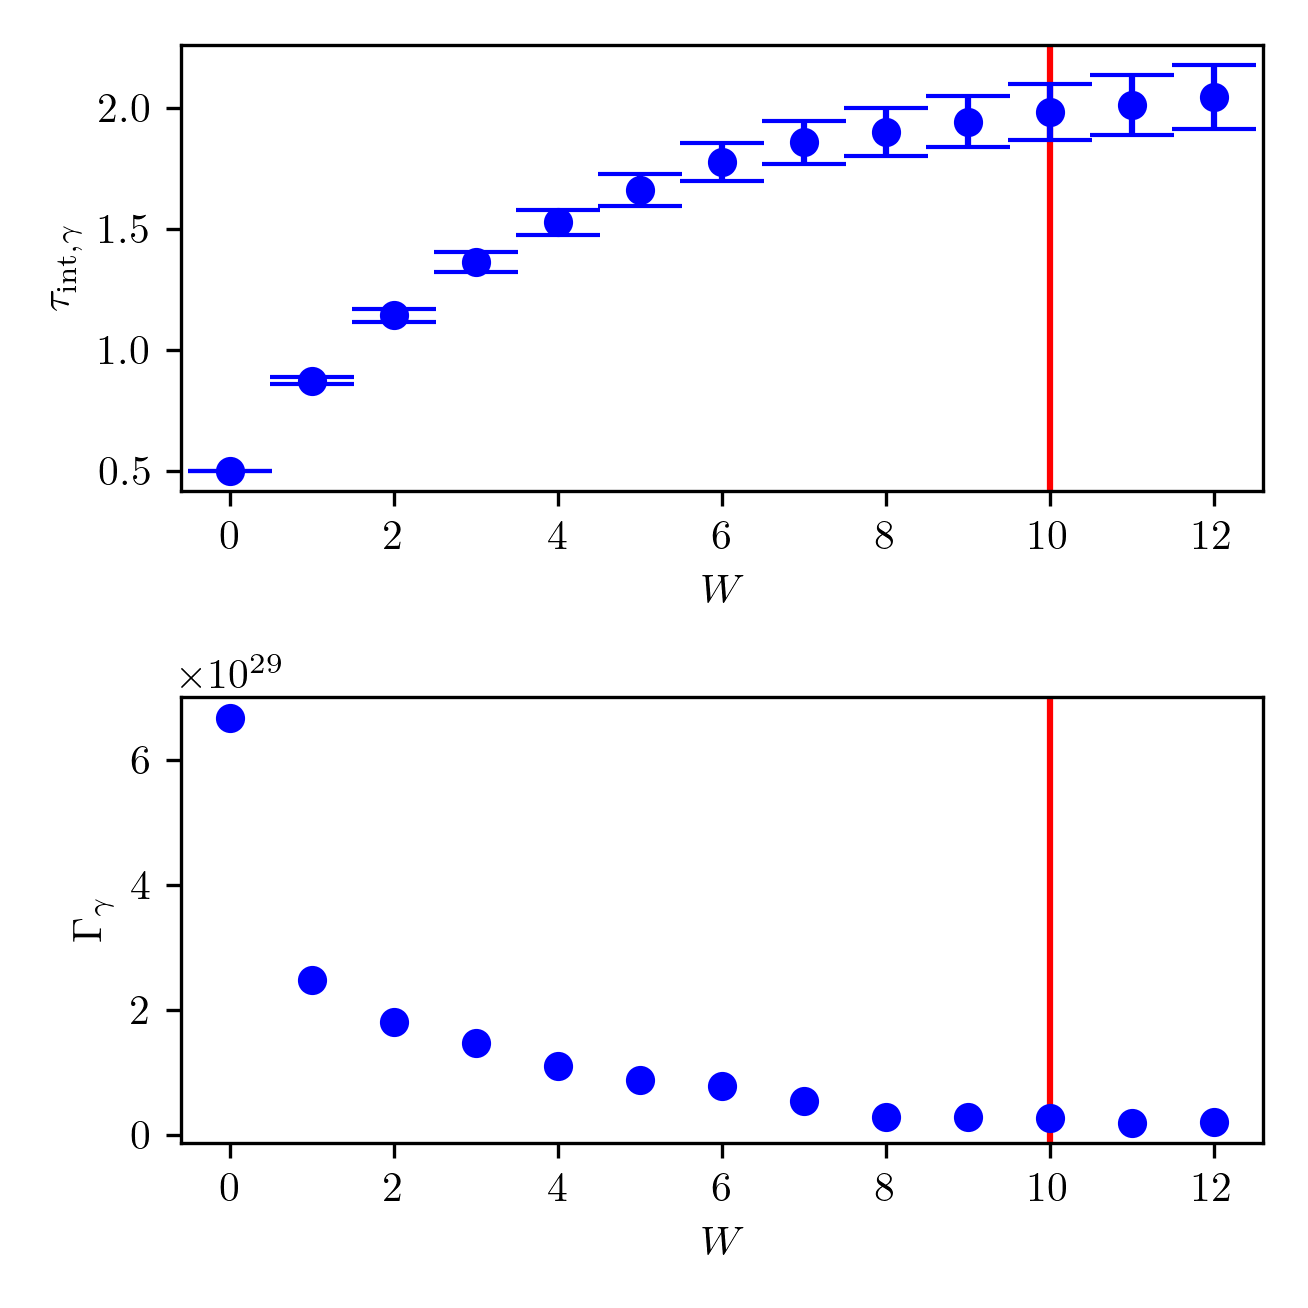
\includegraphics{UwerrTauIntSecO3gam.png}
	\caption[IACT and autocorrelation of samples $\gamma \sim \pi( \cdot| \bm{y})$, for approximated model.]{The IACT $\tau_{\text{int},\gamma}$ at summation windows W as well as the estimated autocorrelation function $\Gamma_{\gamma}$ at lag $t$ of the samples $\gamma \sim \pi( \cdot | \bm{y})$ based on the approximated forward model.
	The estimated IACTs are twice the values provided by~\cite{drikHesse, UwerrM}.}
	\label{fig:IATCSecO3gam}
\end{figure}
\clearpage
\subsection{Eigenvectors of Full Conditional Posterior Precision Matrix}
 \begin{figure}[ht!]
 	\centering
 	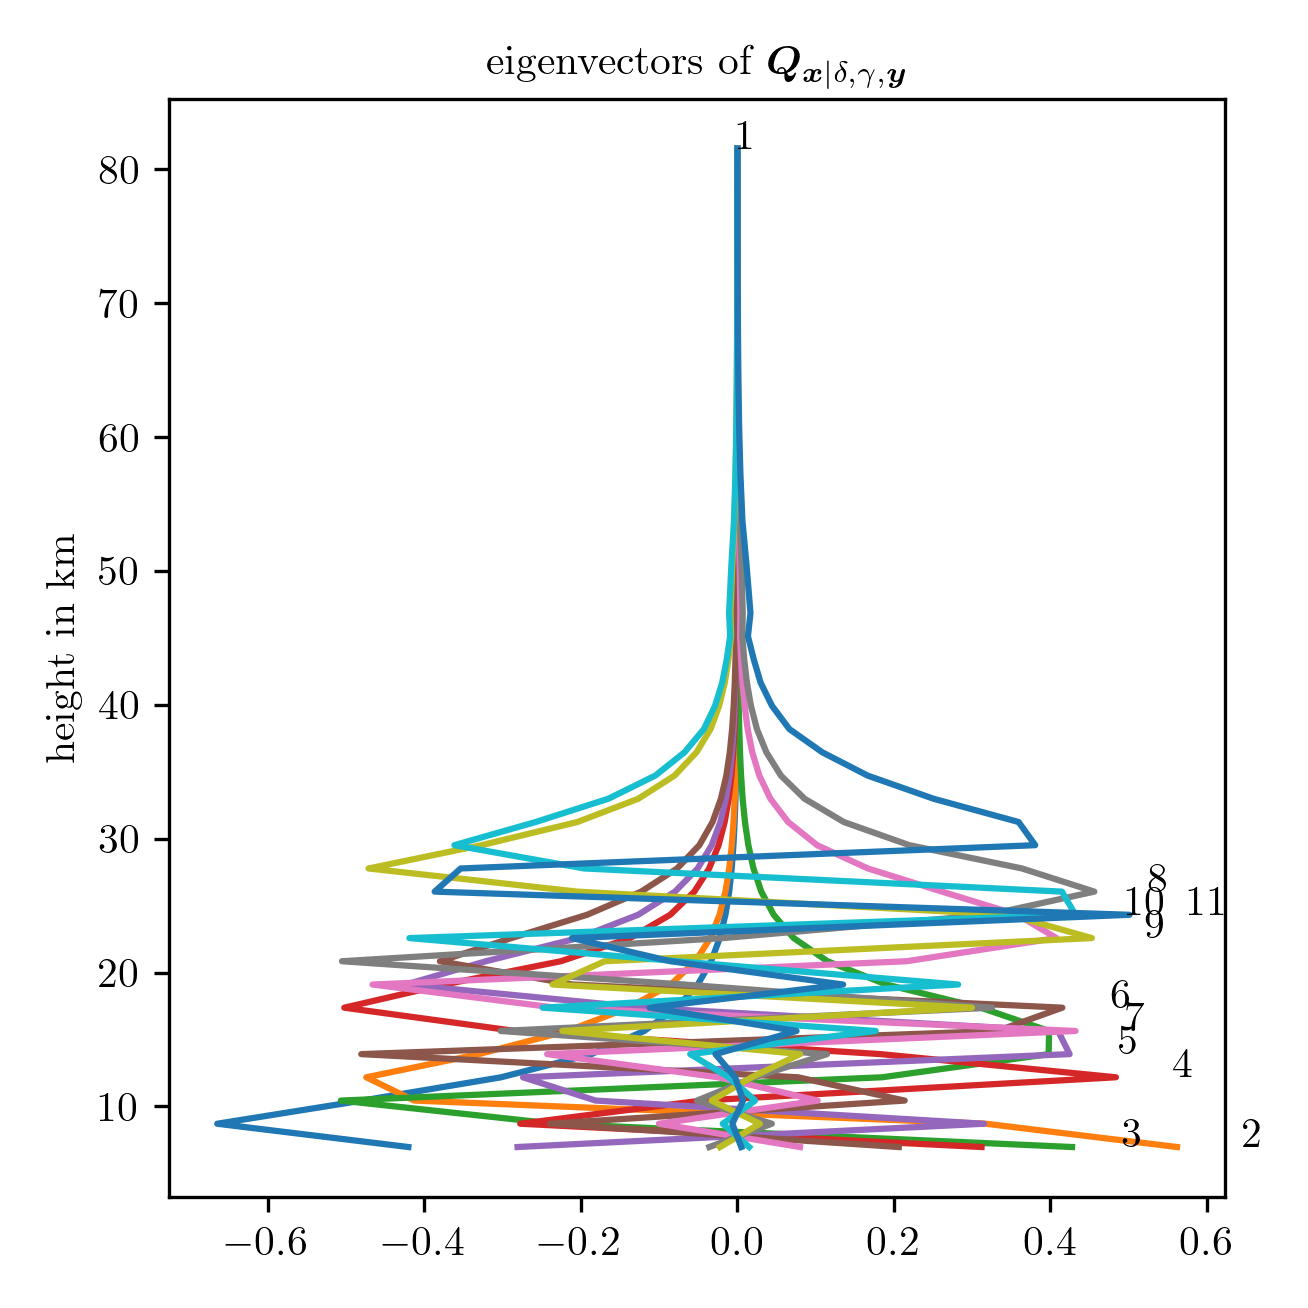
\includegraphics{CovEigVec1.png}
 	\caption[First 12 eigenvectors of conditional precision matrix.]{First 12 eigenvectors corresponding to the in size ordered eigenvalues of the conditional precision matrix $\bm{Q}_{ \bm{x}|\delta, \gamma, \bm{y}}$.
 	The eigenvectors span structures for heights below $35$km.}
 	\label{fig:CovEigVec1}
 \end{figure}
 \begin{figure}[ht!]
 	\centering
 	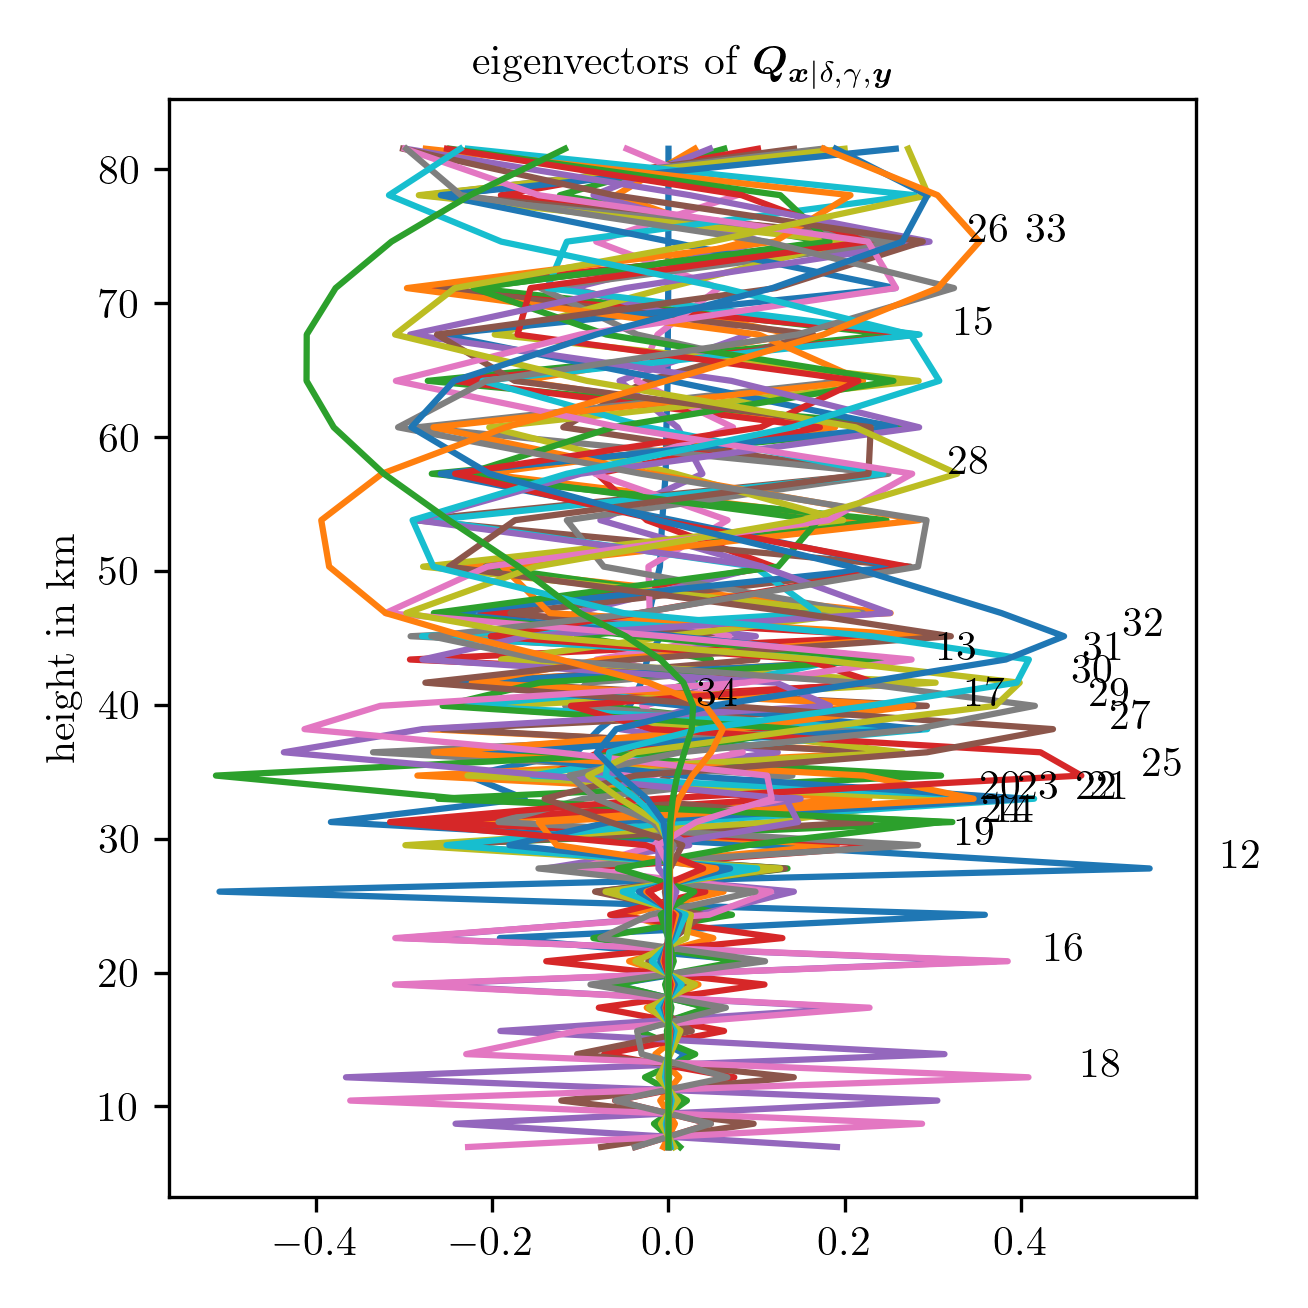
\includegraphics{CovEigVec2.png}
 	\caption[Last 22 eigenvectors of conditional precision matrix.]{Last 22 eigenvectors corresponding to the in size ordered eigenvalues of the conditional precision matrix $\bm{Q}_{ \bm{x}|\delta, \gamma, \bm{y}}$. The eigenvectors mainly represent structures of the prior.}
 	\label{fig:CovEigVec2}
 \end{figure}
\clearpage
\section{Chapter 6}

\subsection{Priors}
\begin{figure}[ht!]
	\centering
	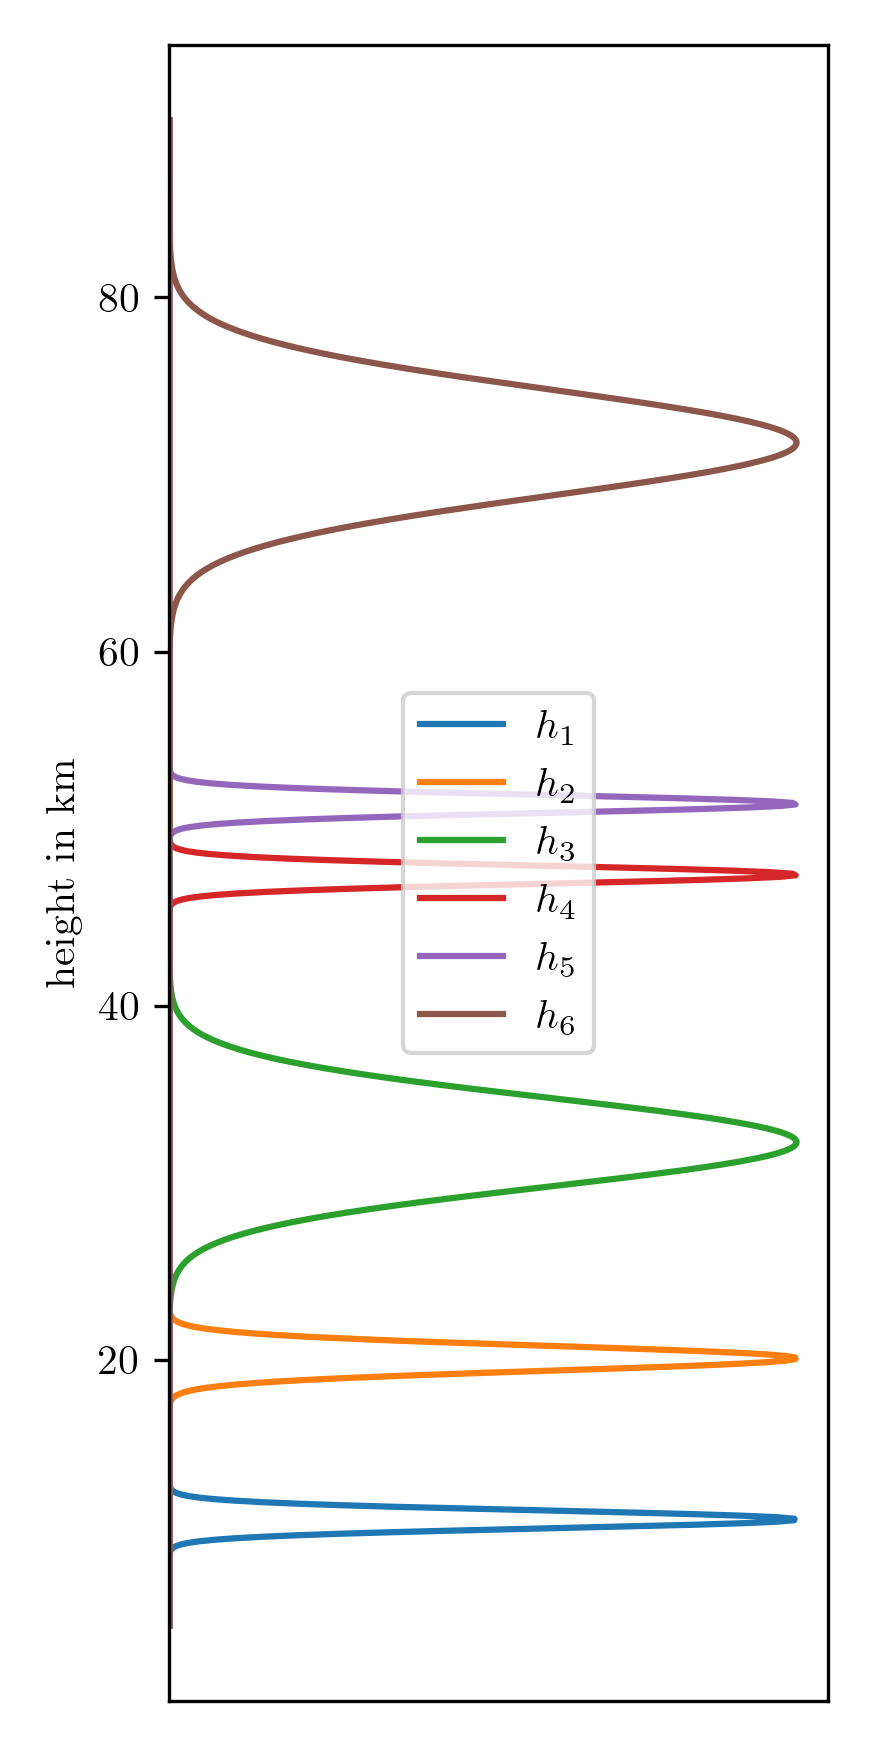
\includegraphics{HeightPriors.png}
	\caption[Prior distributions $\pi(\bm{h_T})$.]{Prior distributions $\pi(\bm{h_T})$, chosen so that they do not overlap and $h_{T,i} < h_{T,i+1}$, for $i = 1, \dots,5$.
	This maintains the structure of the temperature profile in Eq.~\ref{eq:tempFunc}.}
	\label{fig:HeightPriors}
\end{figure} 

\begin{figure}[ht!]
	\centering
	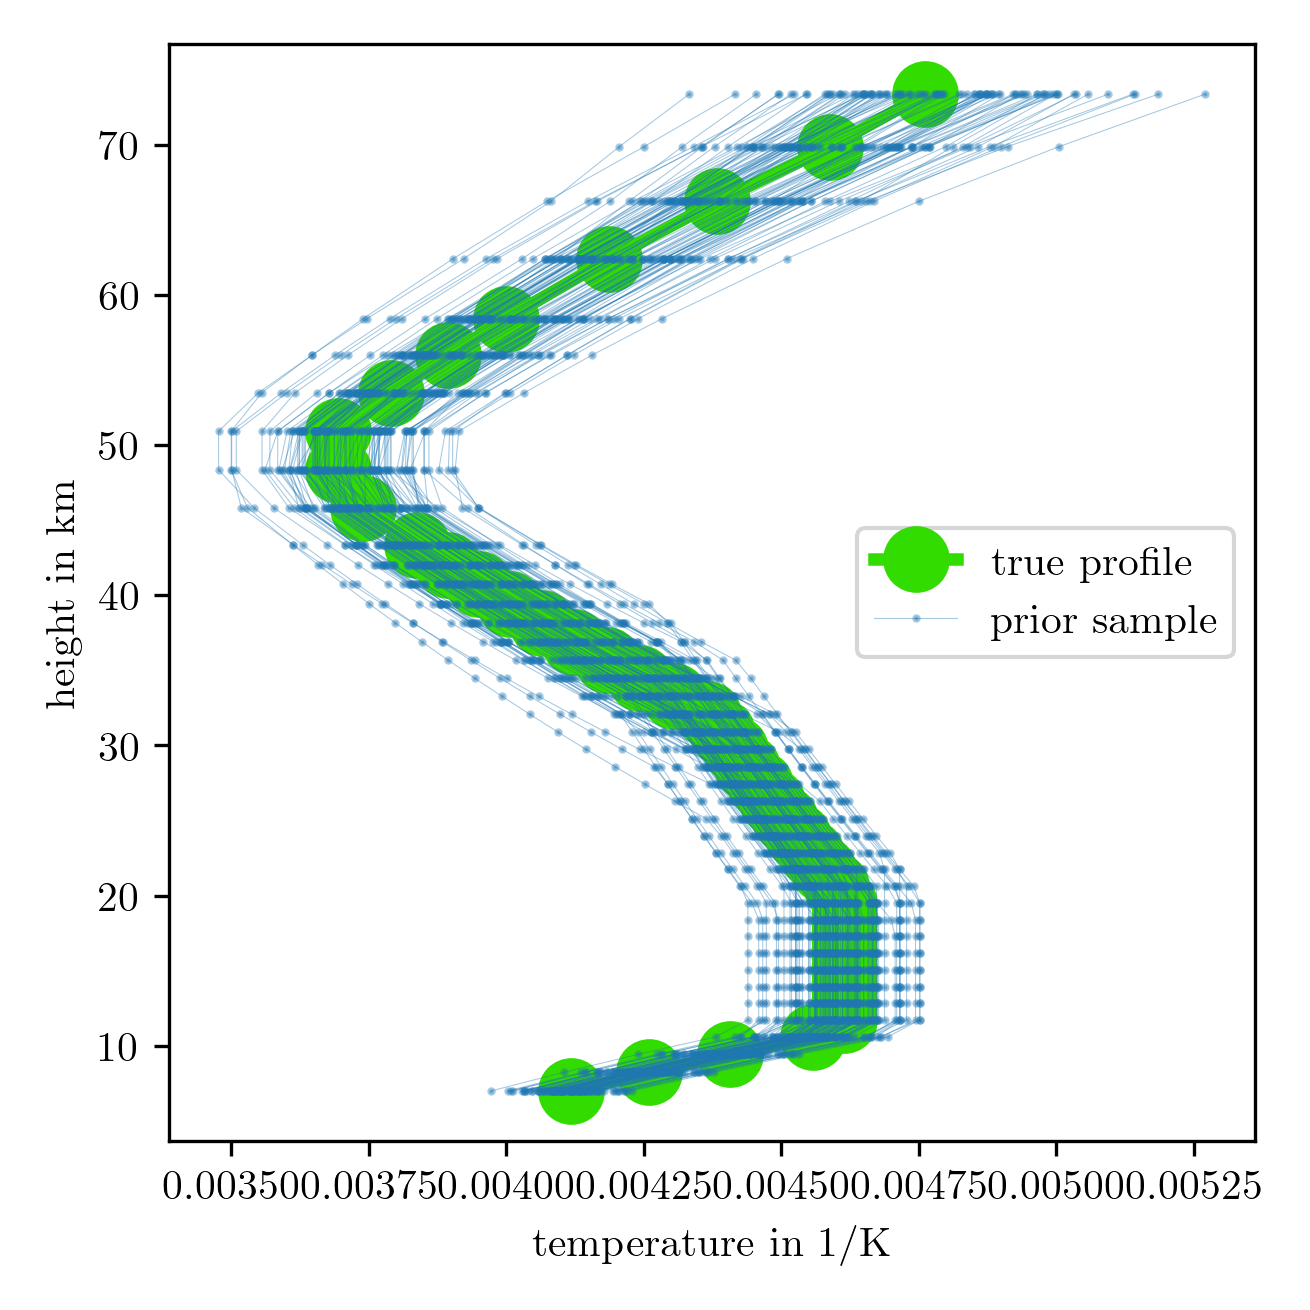
\includegraphics{PriorOverTempPost.png}
	\caption[Prior samples of $1/\bm{T}$]{Prior samples of the inverted temperature profile.}
	\label{fig:OverTempPrior}
\end{figure}
\clearpage

\subsection{Integrated Autocorrelation Time} 
\begin{figure}[ht!]
	\centering
	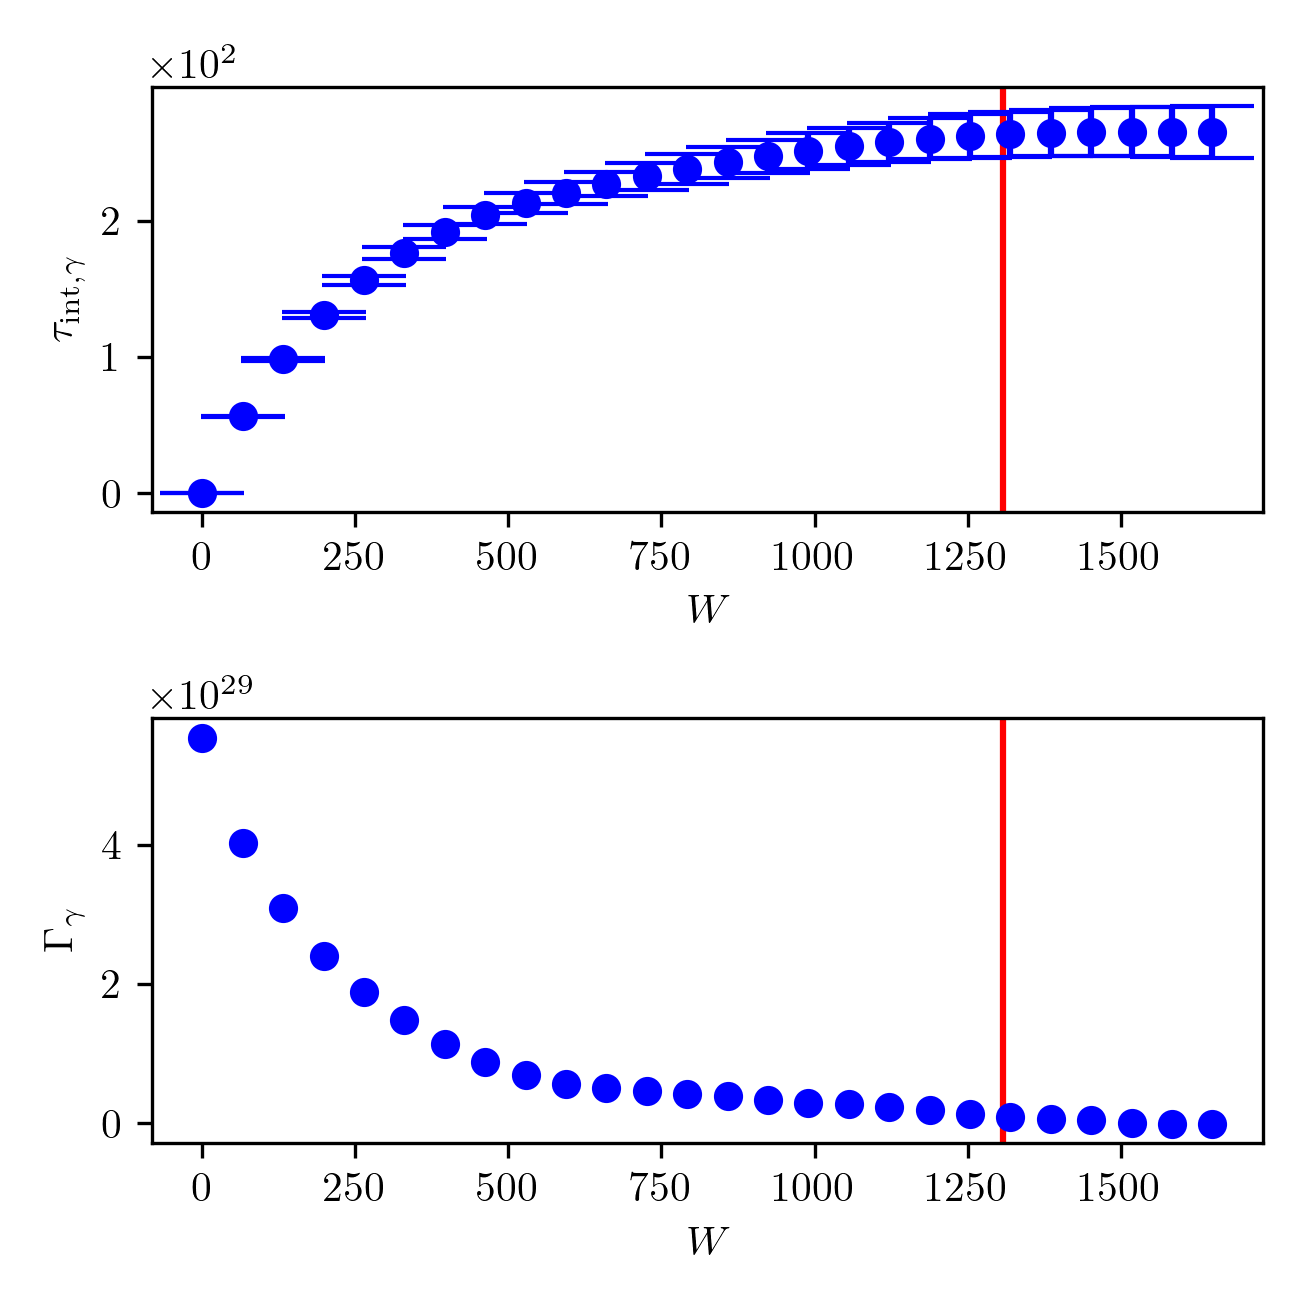
\includegraphics{UwerrTauIntTWalk0.png}
	\caption[IACT and autocorrelation function of samples $\gamma \sim \pi(\cdot|\bm{y})$, for approximated model.]{The IACT $\tau_{\text{int},\gamma }$ at summation windows W and the estimated autocorrelation function $\Gamma_{\gamma }$ at lag $t$ of samples $\gamma  \sim \pi( \cdot| \bm{y})$ from the t-walk for the approximated forward model.
	The estimated IACTs are twice the values provided by~\cite{drikHesse, UwerrM}.}
	\label{fig:TWalkIATC1}
\end{figure}
\begin{figure}[ht!]
	\centering
	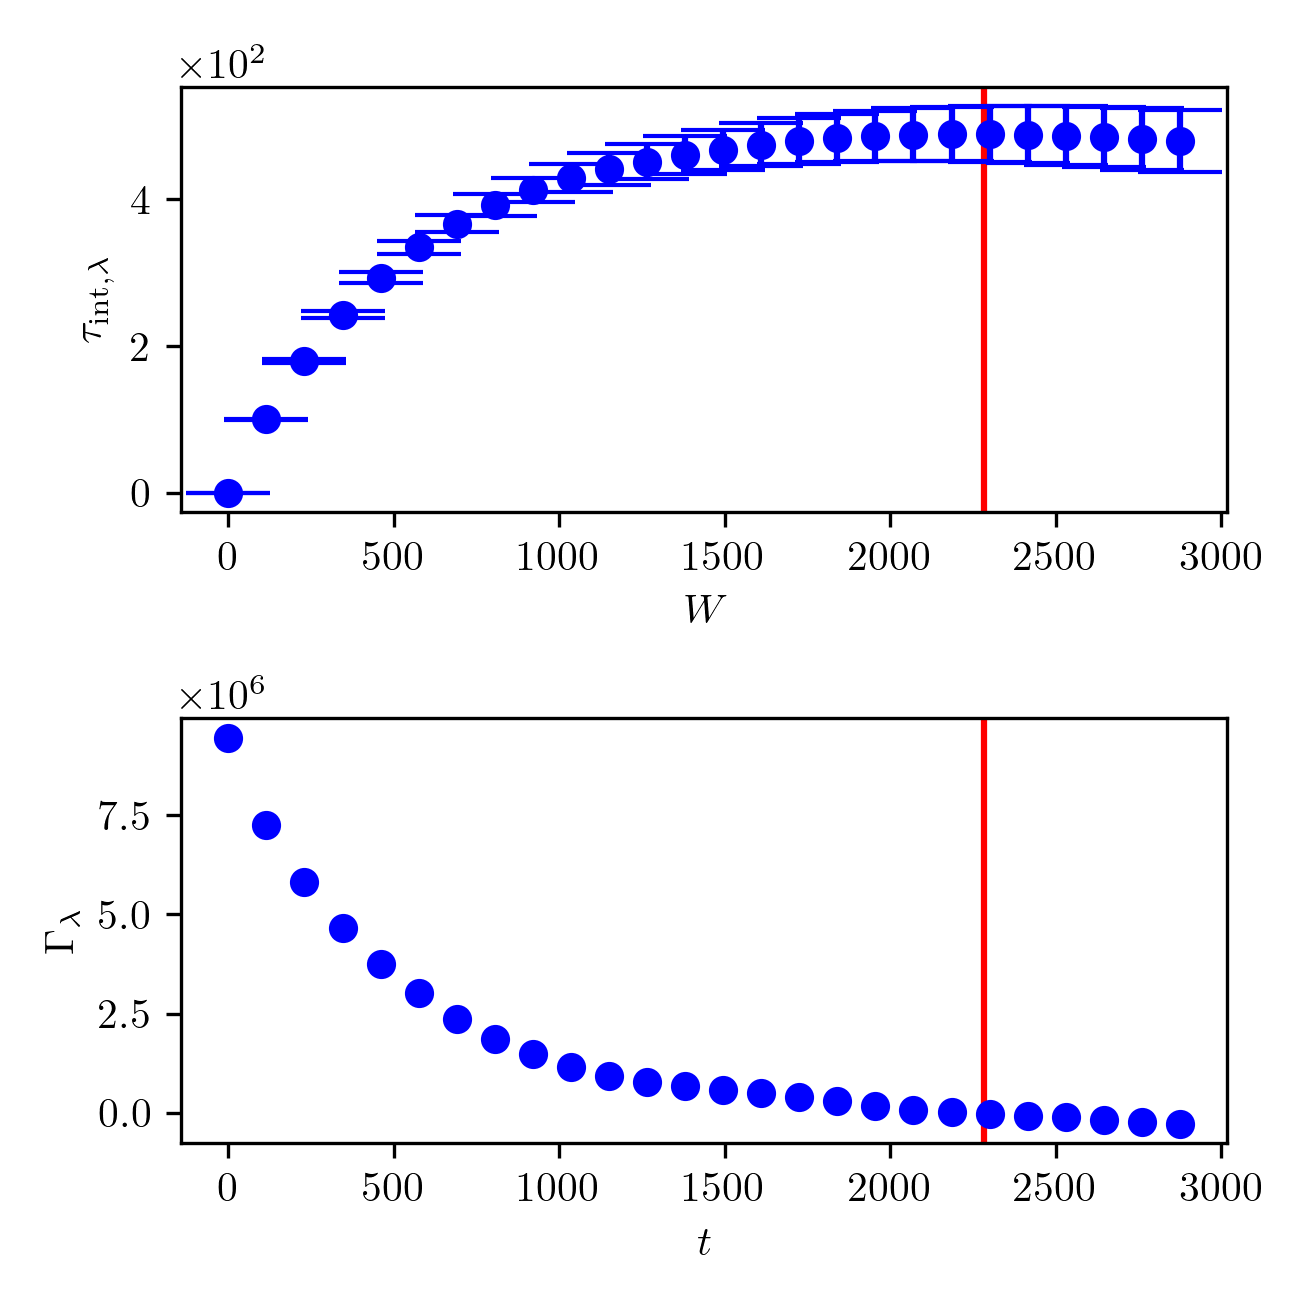
\includegraphics{UwerrTauIntTWalk1.png}
	\caption[IACT and autocorrelation function of samples $\lambda \sim \pi(\cdot|\bm{y})$, for approximated model.]{The IACT $\tau_{\text{int},\lambda}$ at summation windows W and the estimated autocorrelation function $\Gamma_{\lambda}$ at lag $t$ of samples $\lambda \sim \pi( \cdot| \bm{y})$ from the t-walkfor the approximated forward model.
	The estimated IACTs are twice the values provided by~\cite{drikHesse, UwerrM}.}
	\label{fig:TWalkIATC2}
\end{figure}


\begin{figure}[ht!]
	\centering
	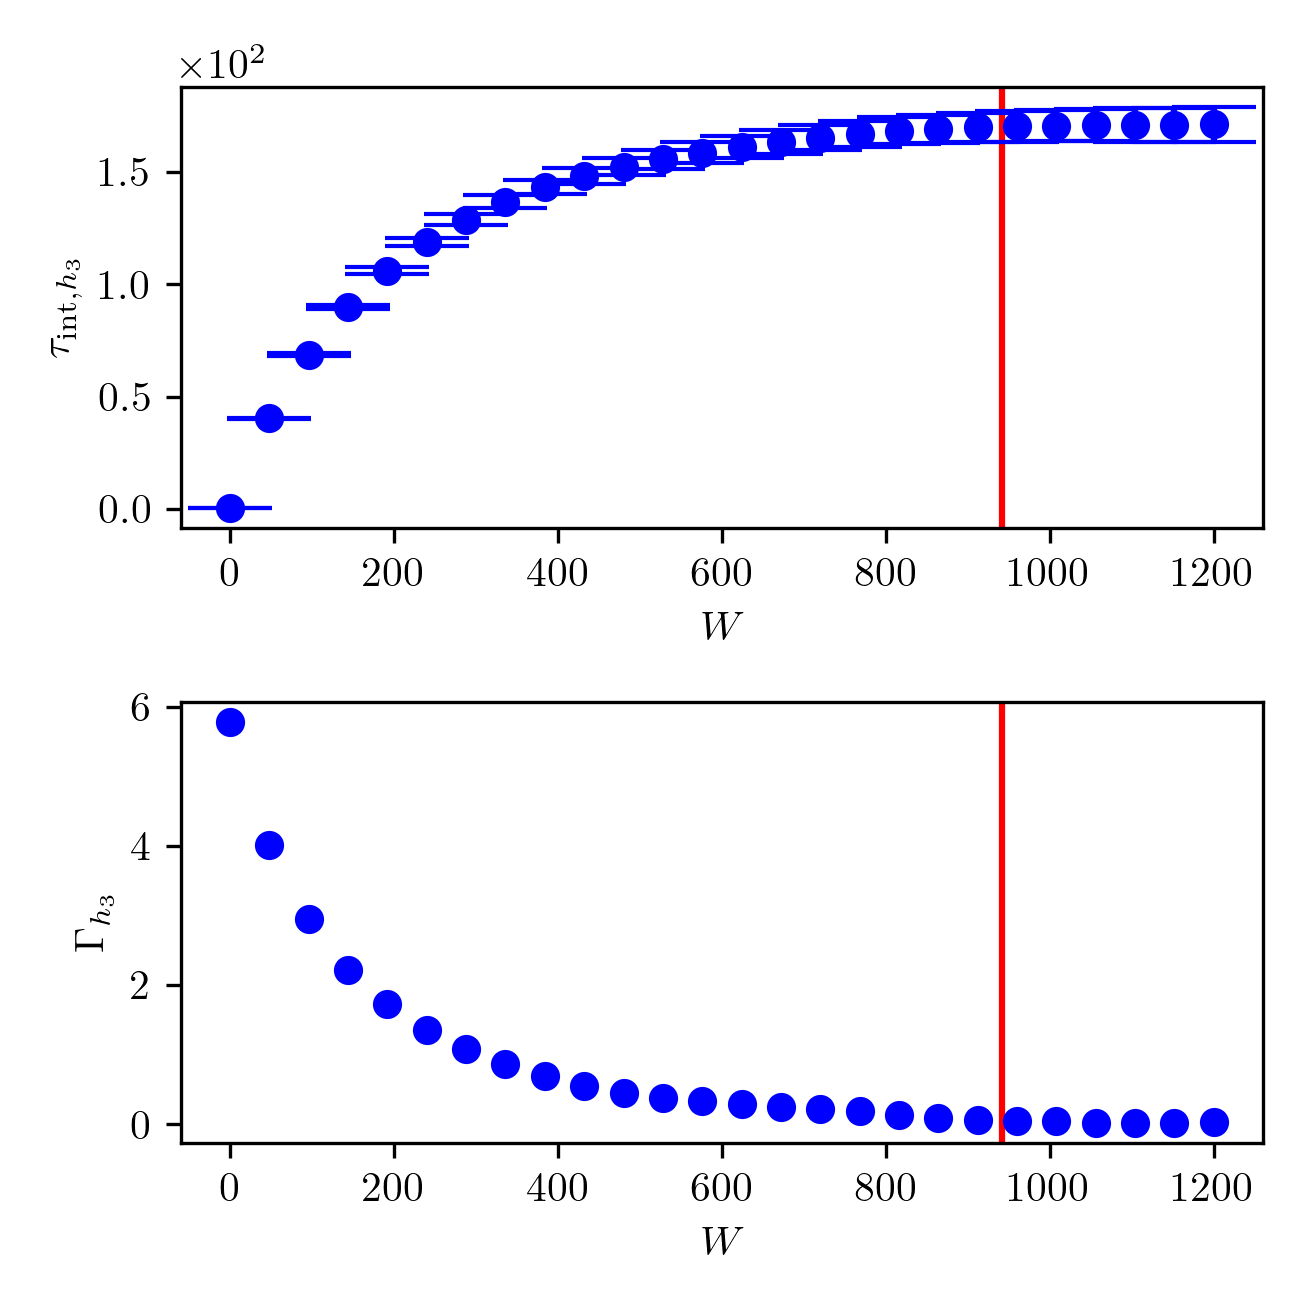
\includegraphics{UwerrTauIntTWalk2.png}
	\caption[IACT and autocorrelation function of samples $b \sim \pi(\cdot|\bm{y})$, for approximated model.]{The IACT $\tau_{\text{int},b}$ at summation windows W and the estimated autocorrelation function $\Gamma_{b}$ at lag $t$ of samples $b \sim \pi( \cdot| \bm{y})$ from the t-walk for the approximated forward model.
	The estimated IACTs are twice the values provided by~\cite{drikHesse, UwerrM}.}
	\label{fig:TWalkIATC3}
\end{figure}


\begin{figure}[ht!]
	\centering
	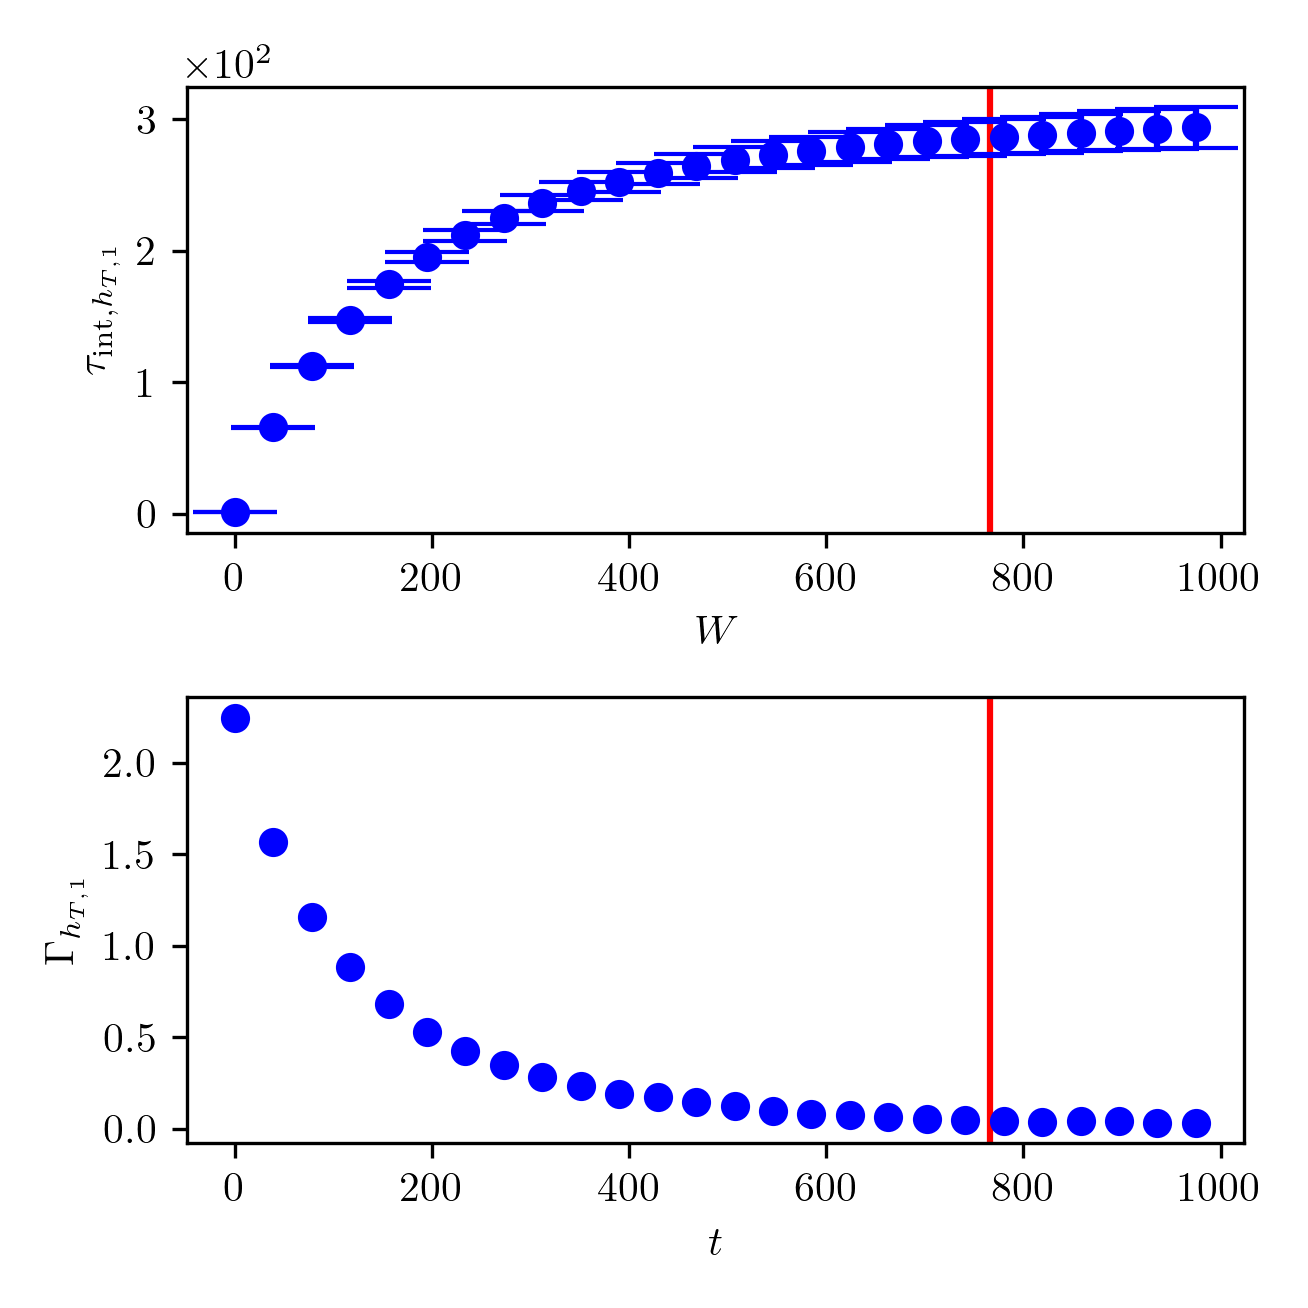
\includegraphics{UwerrTauIntTWalk3.png}
	\caption[IACT and autocorrelation function of samples $h_{T,1} \sim \pi(\cdot|\bm{y})$, for approximated model.]{The IACT $\tau_{\text{int},h_{T,1}}$ at summation windows W and the estimated autocorrelation function $\Gamma_{h_{T,1}}$ at lag $t$ of samples $h_{T,1} \sim \pi( \cdot| \bm{y})$ from the t-walk for the approximated forward model.
	The estimated IACTs are twice the values provided by~\cite{drikHesse, UwerrM}.}
	\label{fig:TWalkIATC4}
\end{figure}


\begin{figure}[ht!]
	\centering
	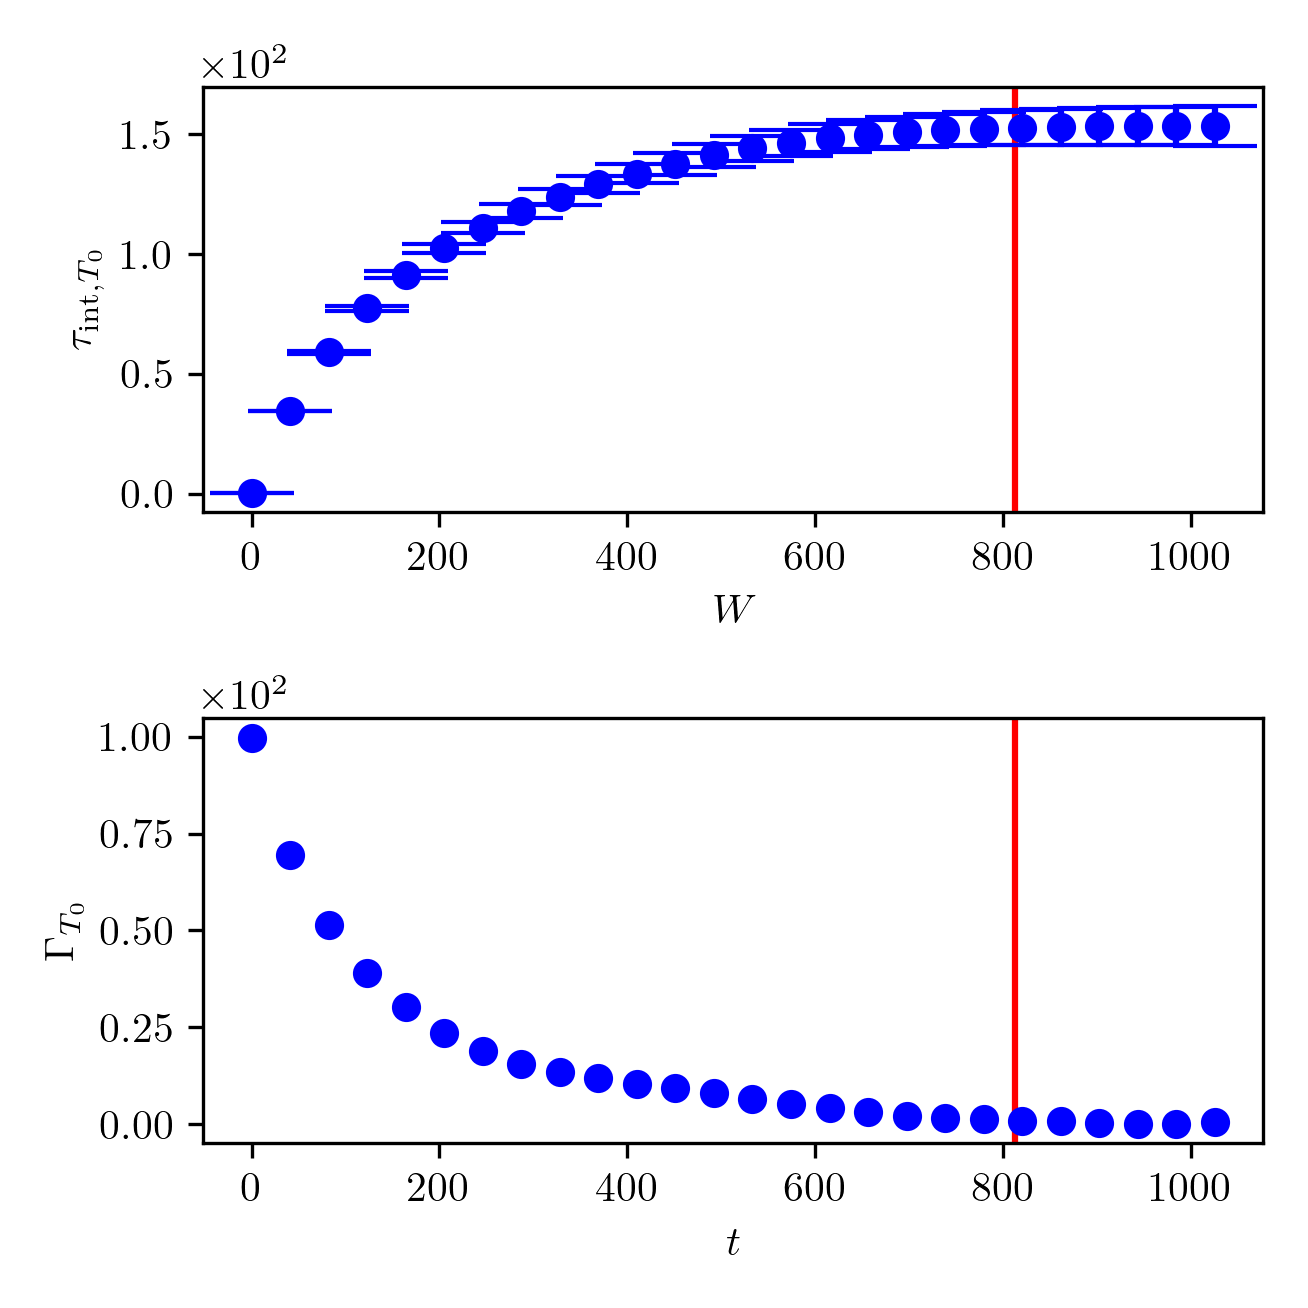
\includegraphics{UwerrTauIntTWalk4.png}
	\caption[IACT and autocorrelation function of samples $T_0  \sim \pi(\cdot|\bm{y})$, for approximated model.]{The IACT $\tau_{\text{int},T_0}$ at summation windows W and the estimated autocorrelation function $\Gamma_{T_0}$ at lag $t$ of samples $T_0 \sim \pi( \cdot| \bm{y})$ from the t-walk for the approximated forward model.
	The estimated IACTs are twice the values provided by~\cite{drikHesse, UwerrM}.}
	\label{fig:TWalkIATC5}
\end{figure}


\begin{figure}[ht!]
	\centering
	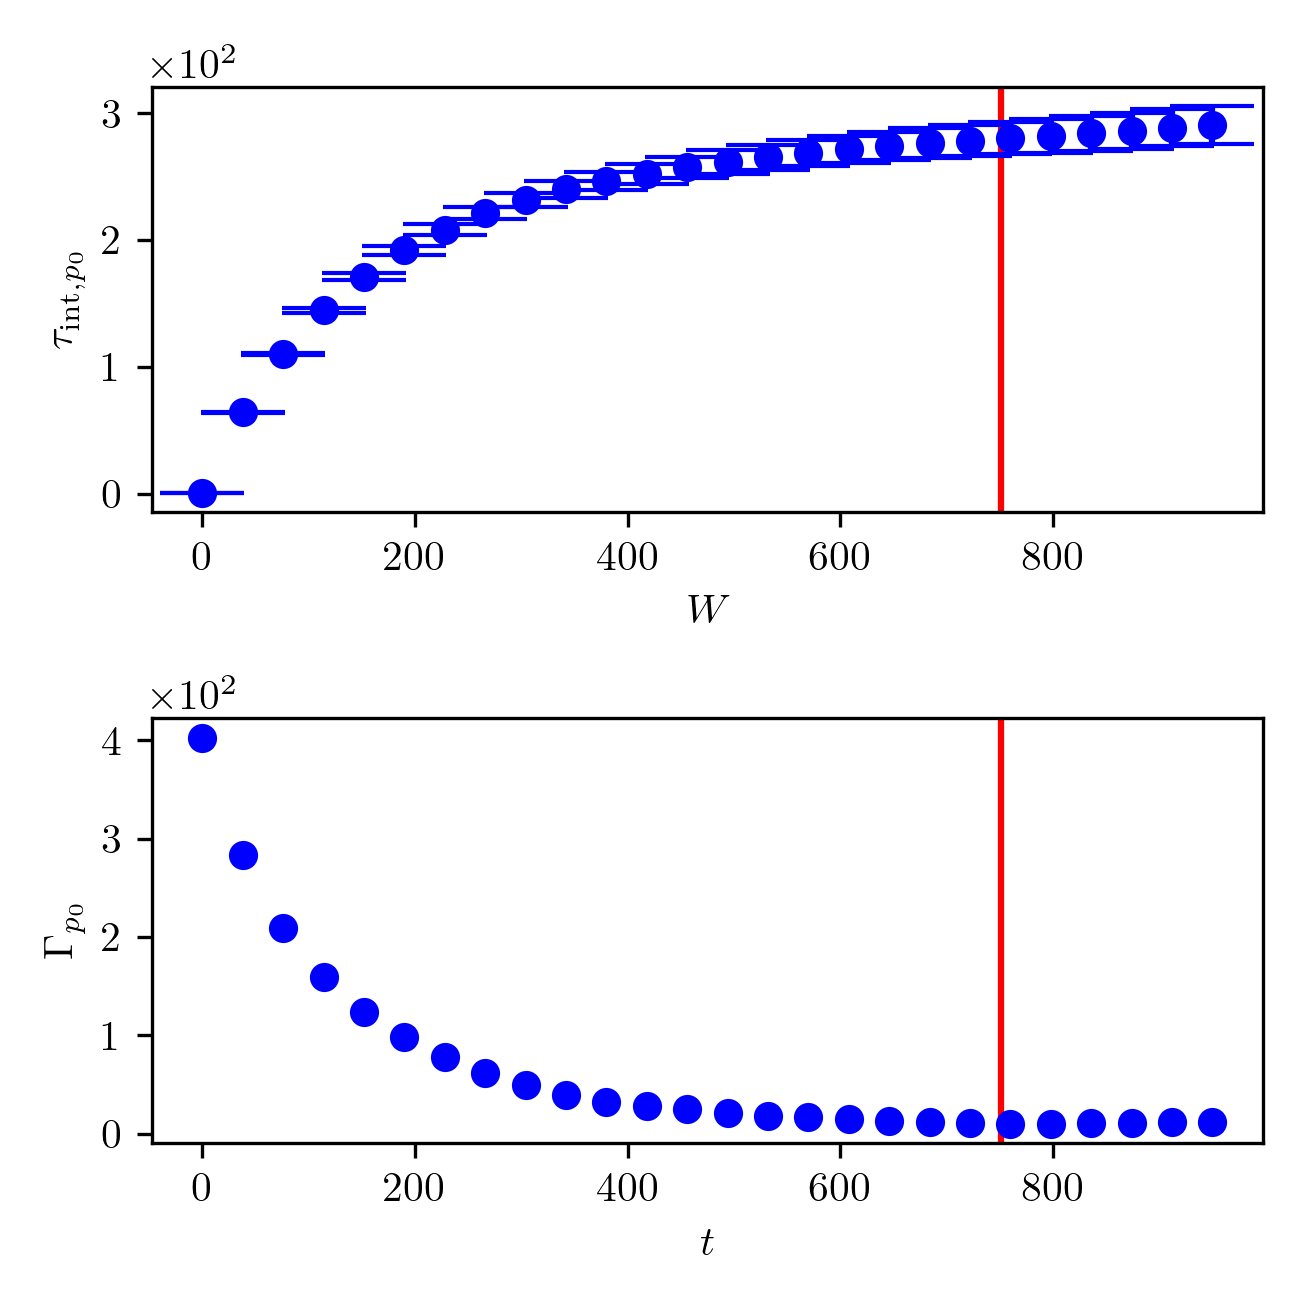
\includegraphics{UwerrTauIntTWalk5.png}
	\caption[IACT and autocorrelation function of samples $p_0 \sim \pi(\cdot|\bm{y})$, for approximated model.]{The IACT $\tau_{\text{int},p_0}$ at summation windows W and the estimated autocorrelation function $\Gamma_{p_0}$ at lag $t$ of samples $p_0 \sim \pi( \cdot| \bm{y})$ from the t-walk for the approximated forward model.
	The estimated IACTs are twice the values provided by~\cite{drikHesse, UwerrM}.}
	\label{fig:TWalkIATC6}
\end{figure}


\begin{figure}[ht!]
	\centering
	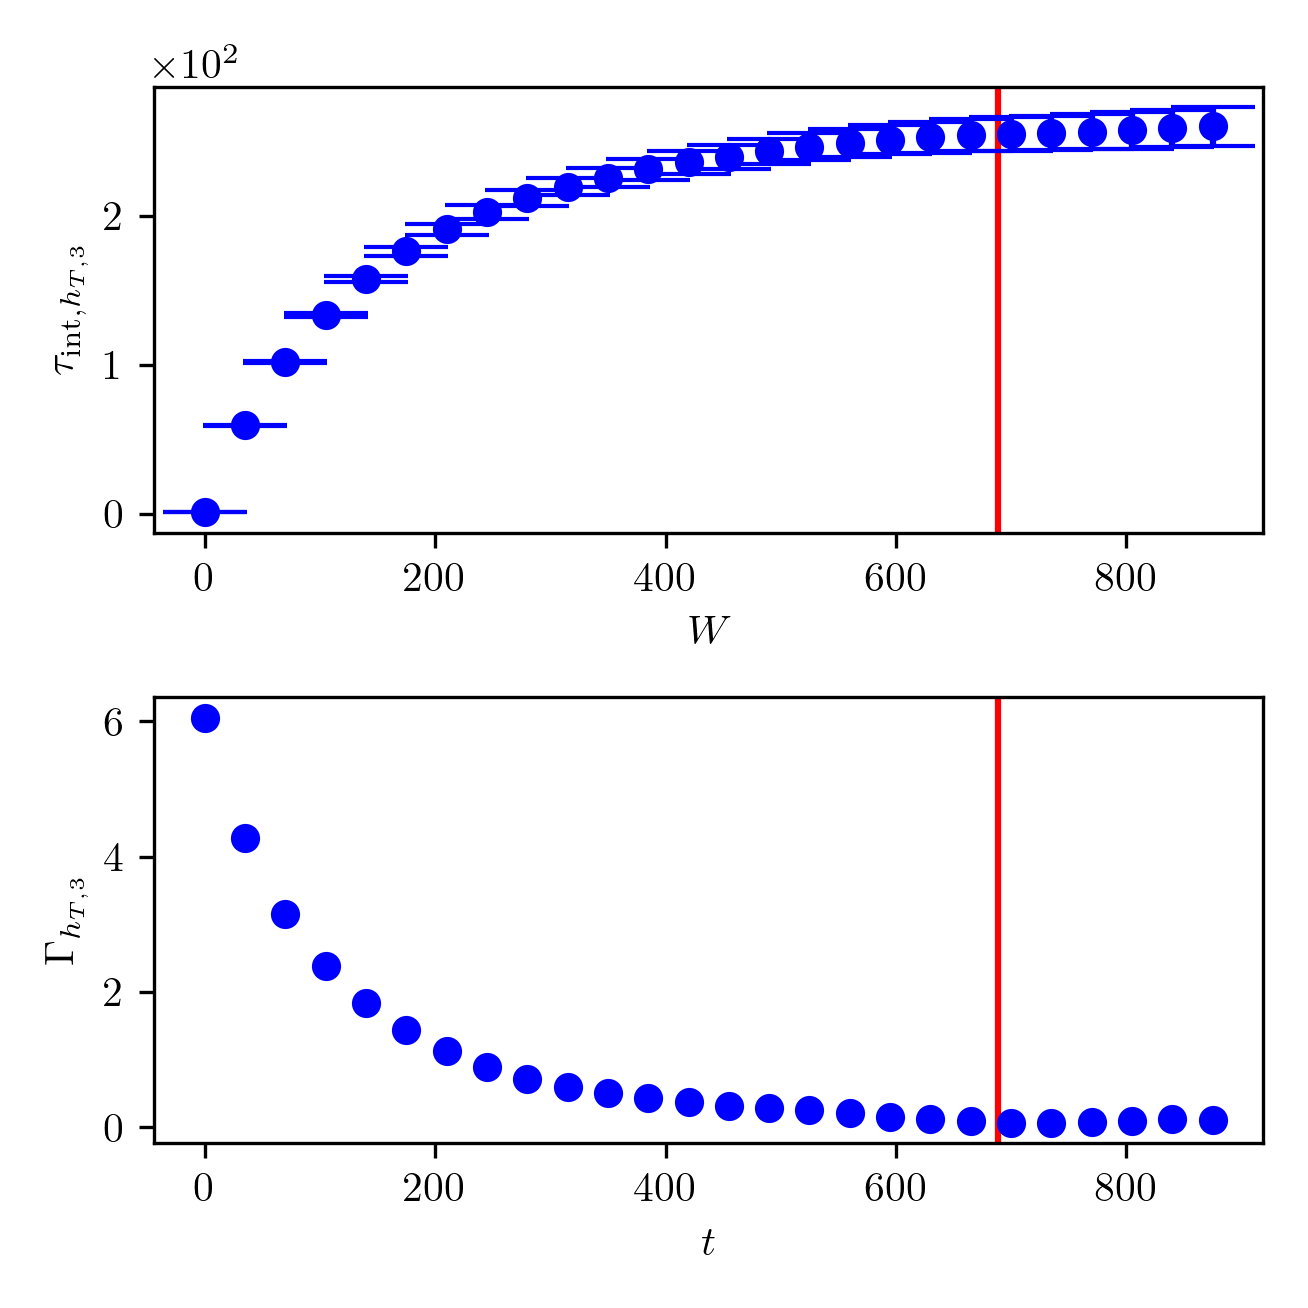
\includegraphics{UwerrTauIntTWalk6.png}
	\caption[IACT and autocorrelation function of samples $h_{T,3} \sim \pi(\cdot|\bm{y})$, for approximated model.]{The IACT $\tau_{\text{int},h_{T,3}}$ at summation windows W and the estimated autocorrelation function $\Gamma_{h_{T,3}}$ at lag $t$ of samples $h_{T,3} \sim \pi( \cdot| \bm{y})$ from the t-walk for the approximated forward model.
	The estimated IACTs are twice the values provided by~\cite{drikHesse, UwerrM}.}
	\label{fig:TWalkIATC7}
\end{figure}

\begin{figure}[ht!]
	\centering
	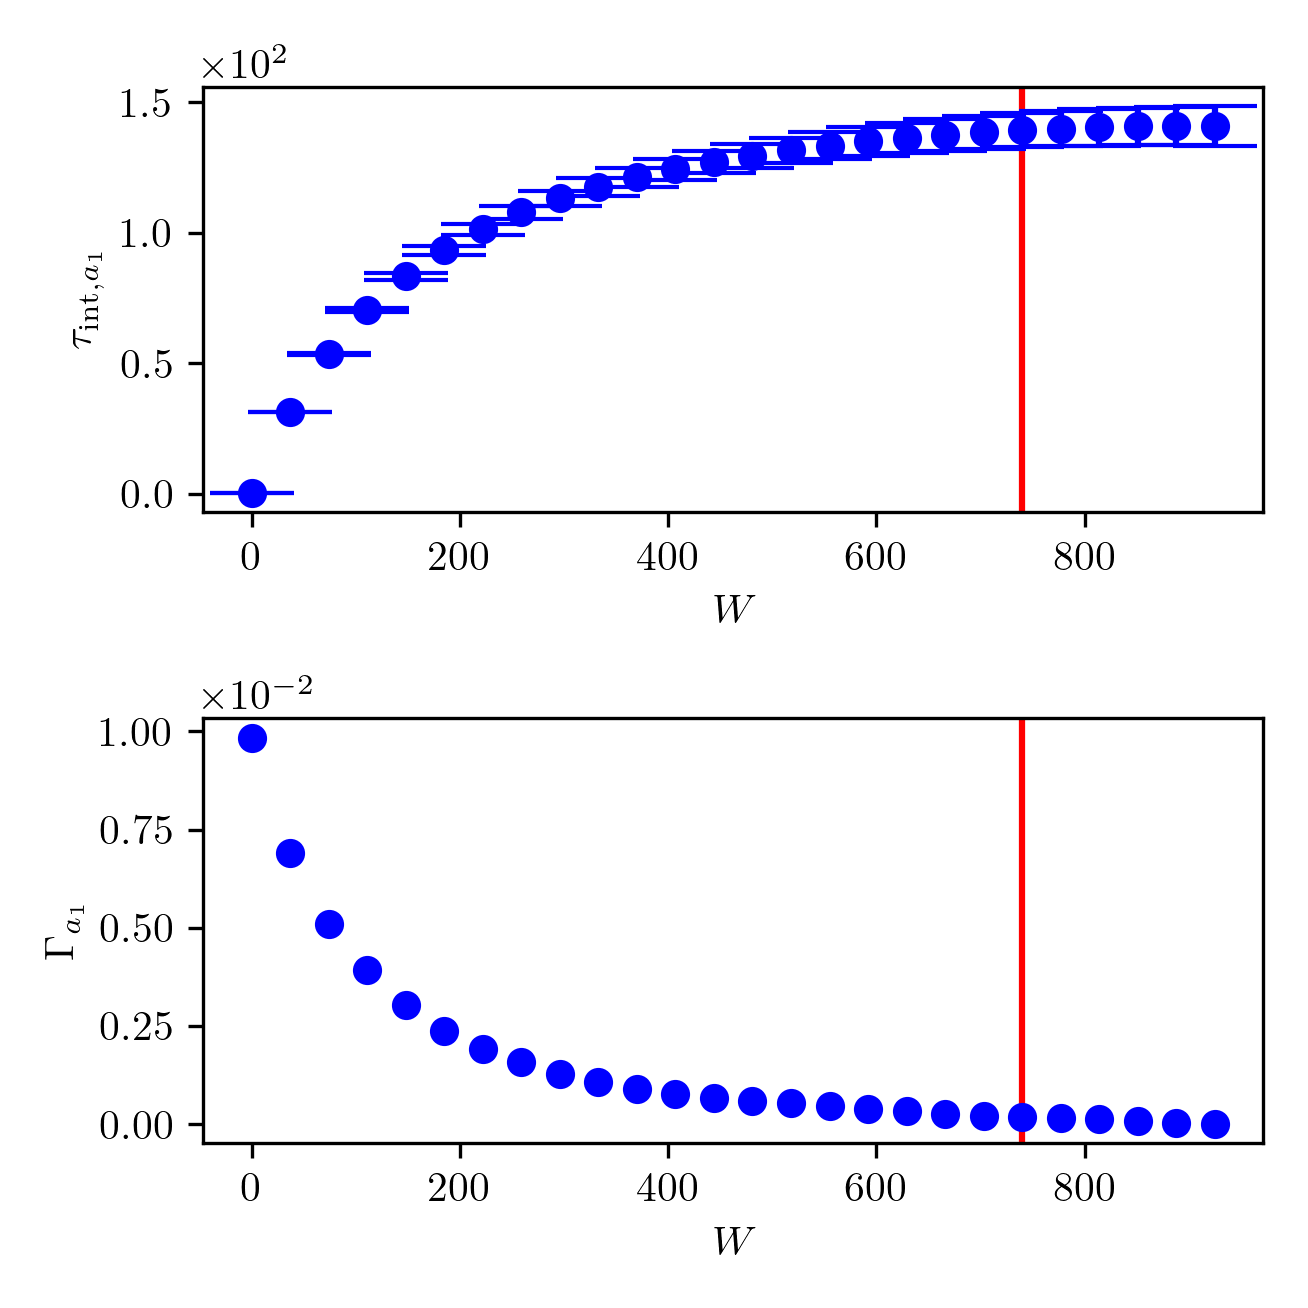
\includegraphics{UwerrTauIntTWalk7.png}
	\caption[IACT and autocorrelation function of samples $a_1 \sim \pi(\cdot|\bm{y})$, for approximated model.]{The IACT $\tau_{\text{int},a_1}$ at summation windows W and the estimated autocorrelation function $\Gamma_{a_1}$ at lag $t$ of samples $a_1 \sim \pi( \cdot| \bm{y})$ from the t-walk for the approximated forward model.
	The estimated IACTs are twice the values provided by~\cite{drikHesse, UwerrM}.}
	\label{fig:TWalkIATC8}
\end{figure}


\begin{figure}[ht!]
	\centering
	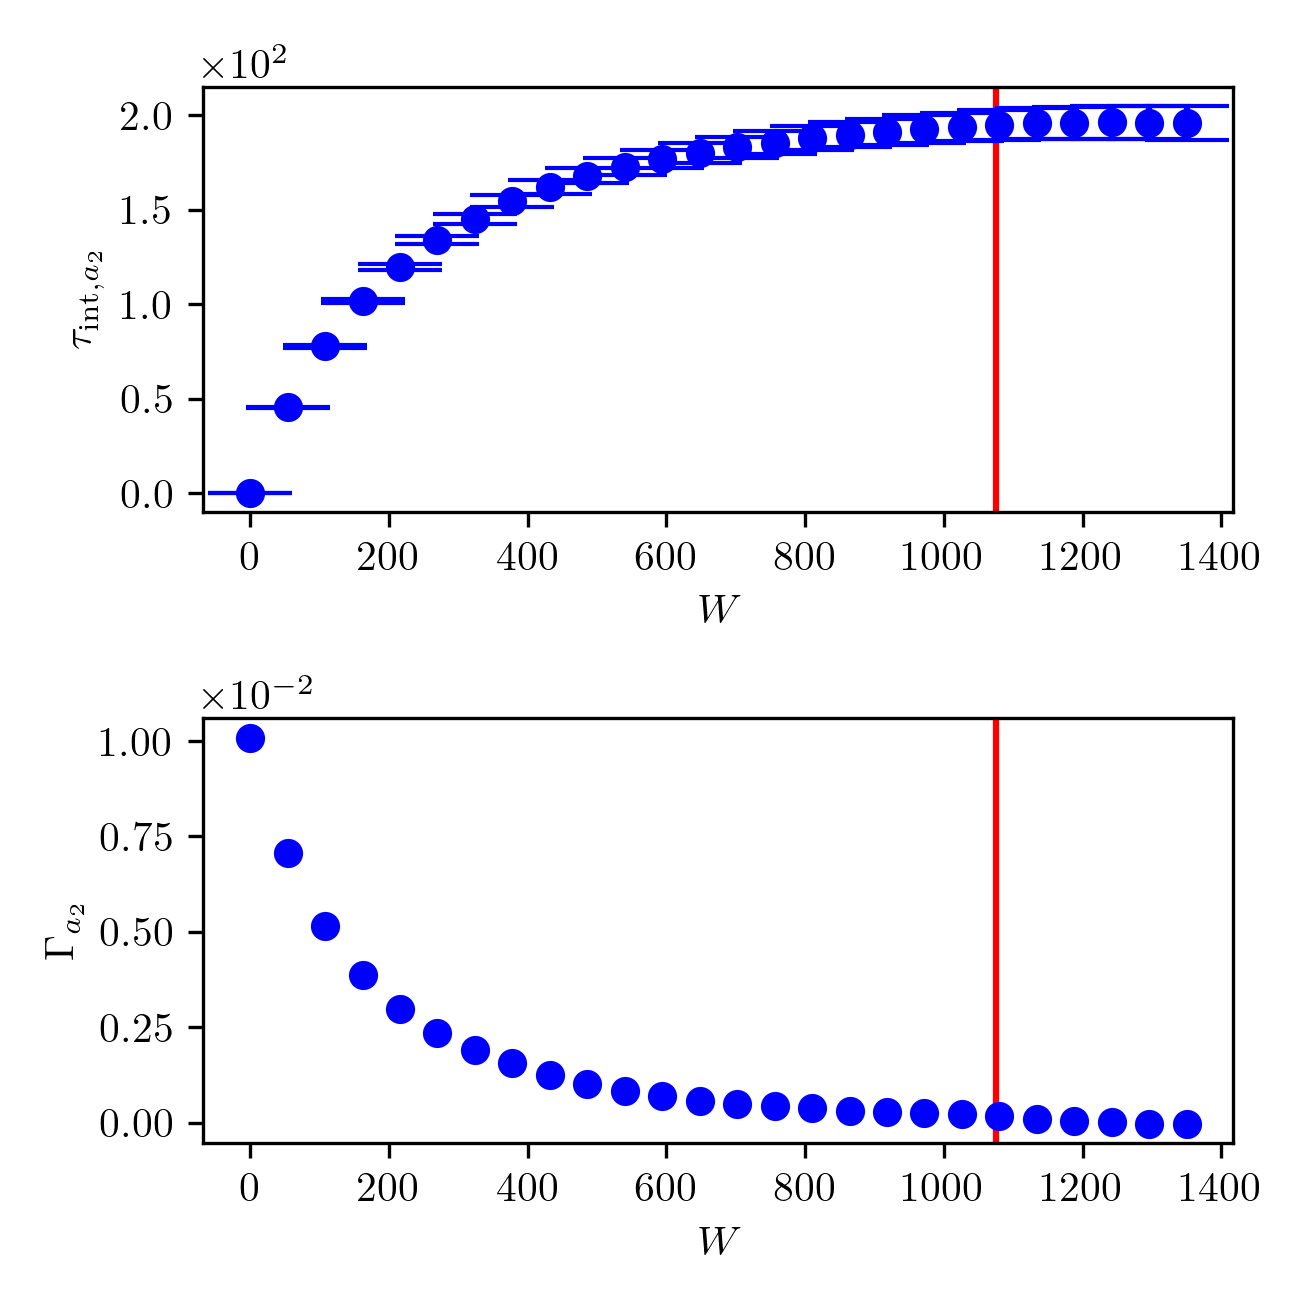
\includegraphics{UwerrTauIntTWalk8.png}
	\caption[IACT and autocorrelation function of samples $h_{T,2} \sim \pi(\cdot|\bm{y})$, for approximated model.]{The IACT $\tau_{\text{int},h_{T,2}}$ at summation windows W and the estimated autocorrelation function $\Gamma_{h_{T,2}}$ at lag $t$ of samples $h_{T,2} \sim \pi( \cdot | \bm{y})$ from the t-walk for the approximated forward model.
	The estimated IACTs are twice the values provided by~\cite{drikHesse, UwerrM}.}
	\label{fig:TWalkIATC9}
\end{figure}


\begin{figure}[ht!]
	\centering
	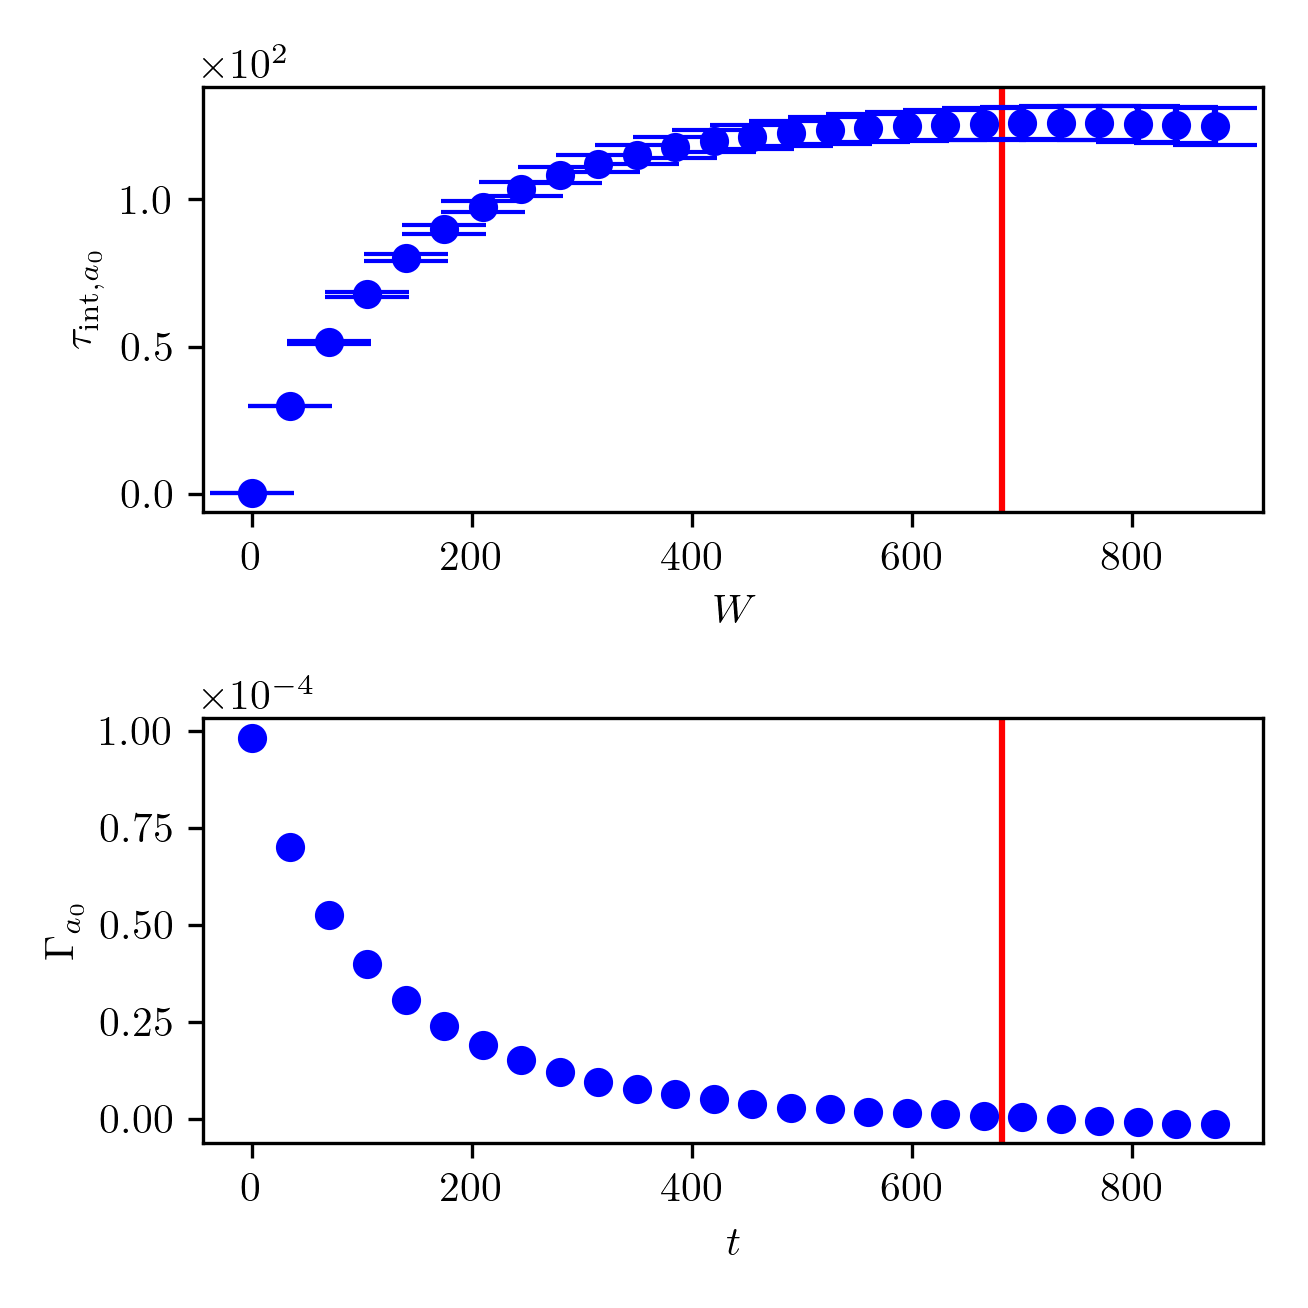
\includegraphics{UwerrTauIntTWalk9.png}
	\caption[IACT and autocorrelation function of samples $a_0 \sim \pi(\cdot|\bm{y})$, for approximated model.]{The IACT $\tau_{\text{int},a_0}$ at summation windows W and the estimated autocorrelation function $\Gamma_{a_0}$ at lag $t$ of samples $a_0 \sim \pi( \cdot| \bm{y})$ from the t-walk for the approximated forward model.
	The estimated IACTs are twice the values provided by~\cite{drikHesse, UwerrM}.}
\end{figure}

\begin{figure}[ht!]
	\centering
	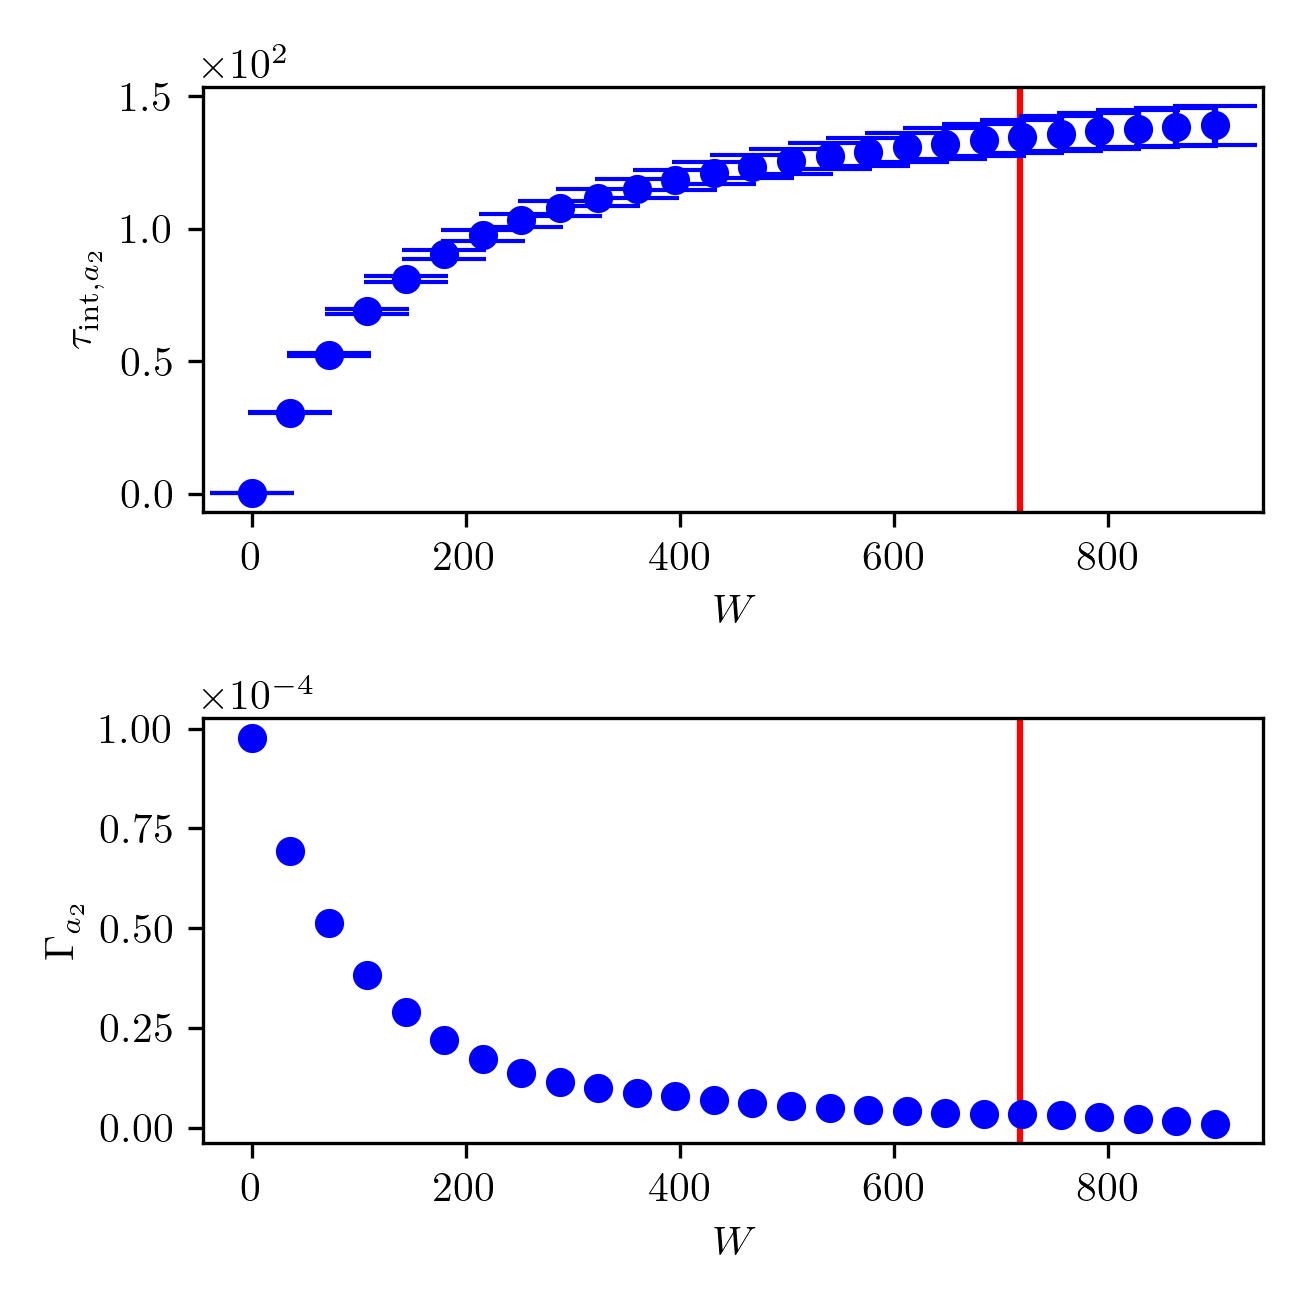
\includegraphics{UwerrTauIntTWalk10.png}
	\caption[IACT and autocorrelation function of samples $a_2 \sim \pi(\cdot|\bm{y})$, for approximated model.]{The IACT $\tau_{\text{int},a_2}$ at summation windows W and the estimated autocorrelation function $\Gamma_{a_2}$ at lag $t$ of samples $a_2 \sim \pi( \cdot | \bm{y})$ from the t-walk for the approximated forward model.
		he estimated IACTs are twice the values provided by~\cite{drikHesse, UwerrM}.}
	\label{fig:TWalkIATC11}
\end{figure}


\begin{figure}[ht!]
	\centering
	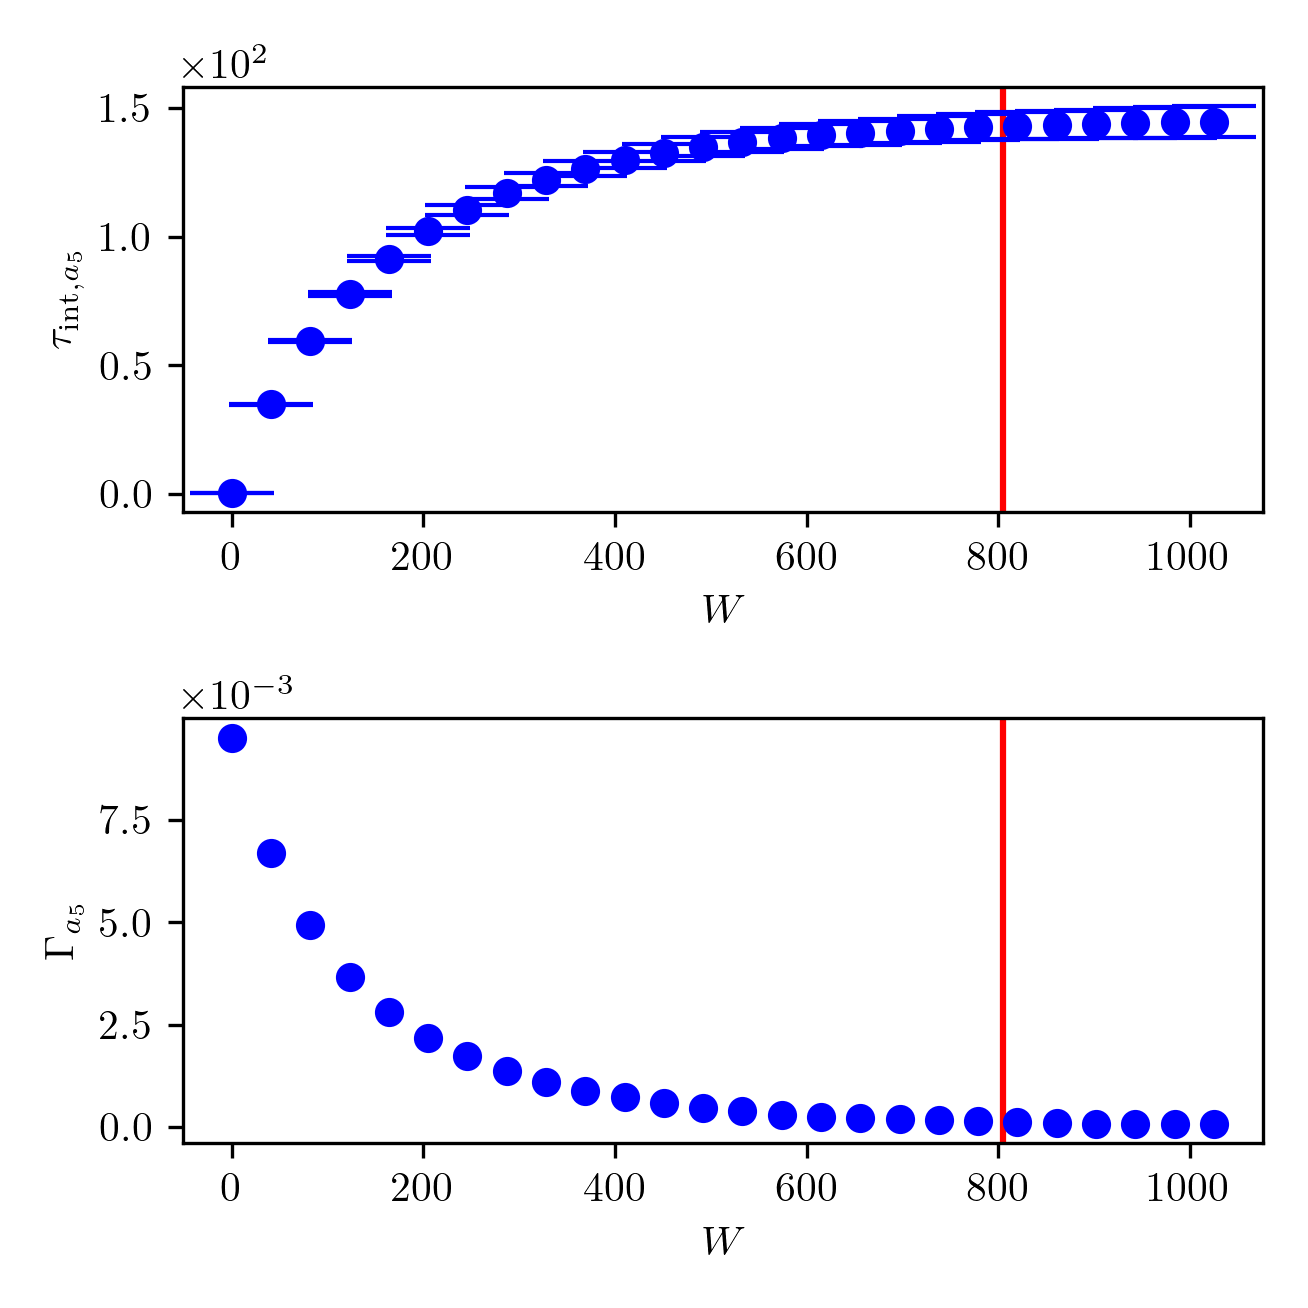
\includegraphics{UwerrTauIntTWalk11.png}
	\caption[IACT and autocorrelation function of samples $a_3 \sim \pi(\cdot|\bm{y})$, for approximated model.]{The IACT $\tau_{\text{int},a_3}$ at summation windows W and the estimated autocorrelation function $\Gamma_{a_3}$ at lag $t$ of samples $a_3 \sim \pi( \cdot| \bm{y})$ from the t-walk for the approximated forward model.
	The estimated IACTs are twice the values provided by~\cite{drikHesse, UwerrM}.}
	\label{fig:TWalkIATC12}
\end{figure}
\begin{figure}[ht!]
	\centering
	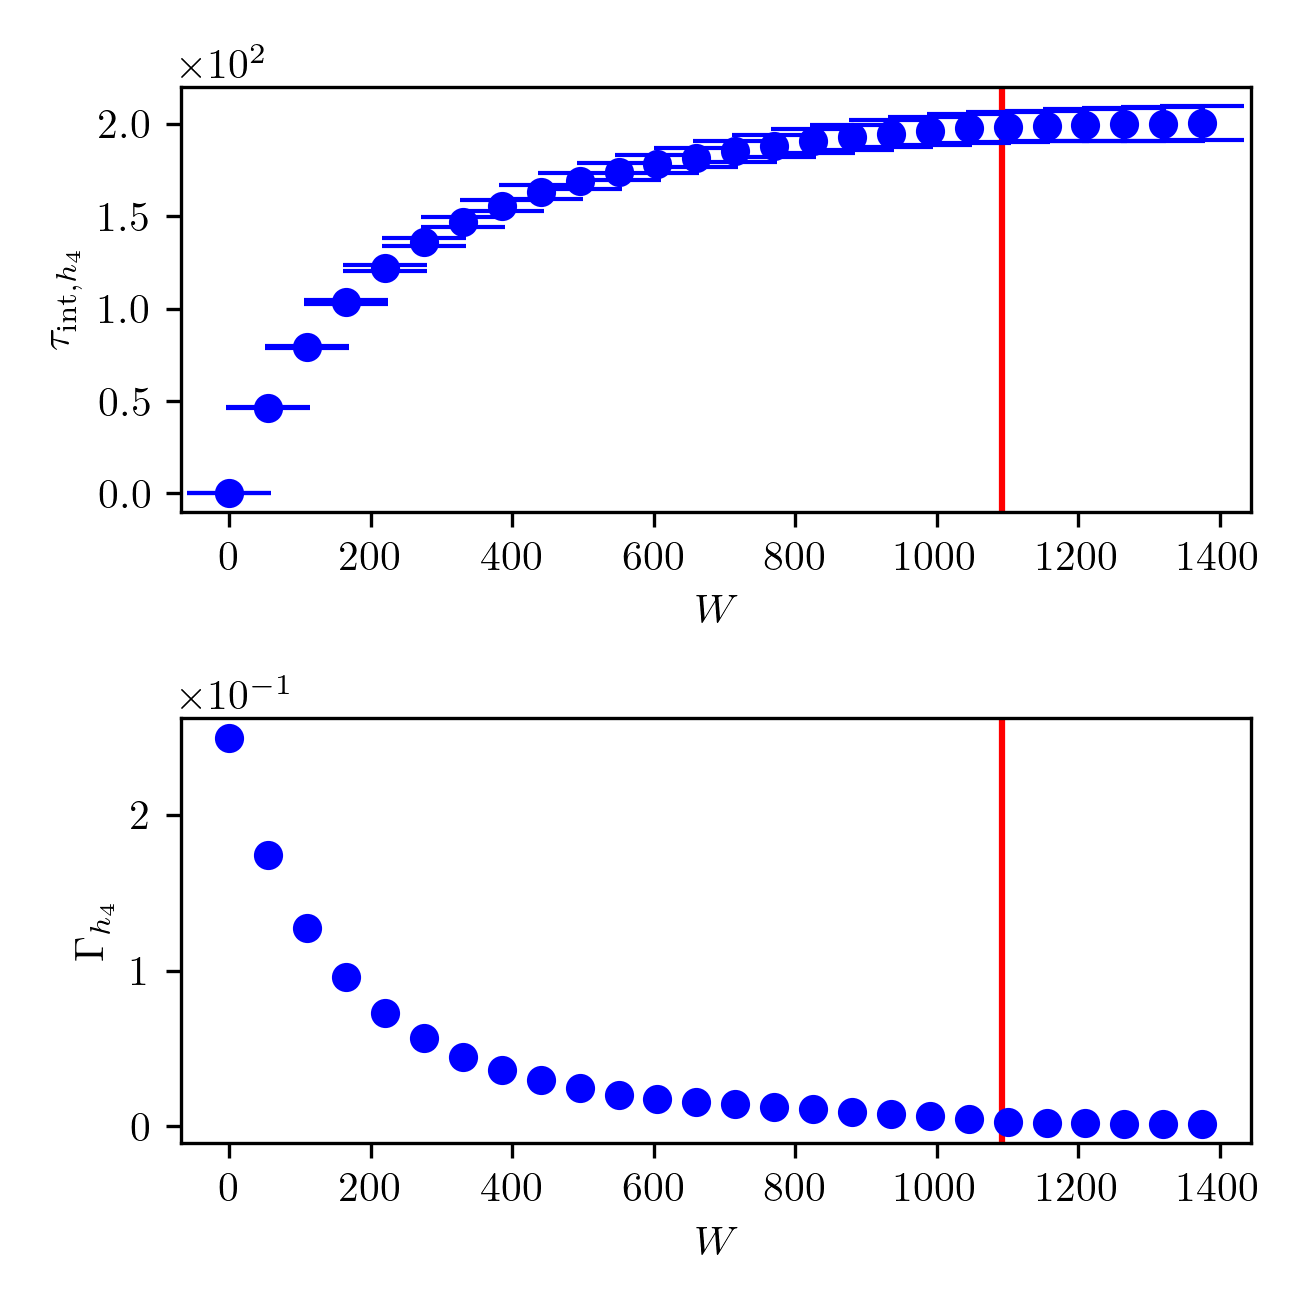
\includegraphics{UwerrTauIntTWalk12.png}
	\caption[IACT and autocorrelation function of samples $h_{T,4} \sim \pi(\cdot|\bm{y})$, for approximated model.]{The IACT $\tau_{\text{int},h_{T,4}}$ at summation windows W and the estimated autocorrelation function $\Gamma_{h_{T,4}}$ at lag $t$ of samples $h_{T,4} \sim \pi( \cdot| \bm{y})$ from the t-walk for the approximated forward model.
	The estimated IACTs are twice the values provided by~\cite{drikHesse, UwerrM}.}
	\label{fig:TWalkIATC13}
\end{figure}
\begin{figure}[ht!]
	\centering
	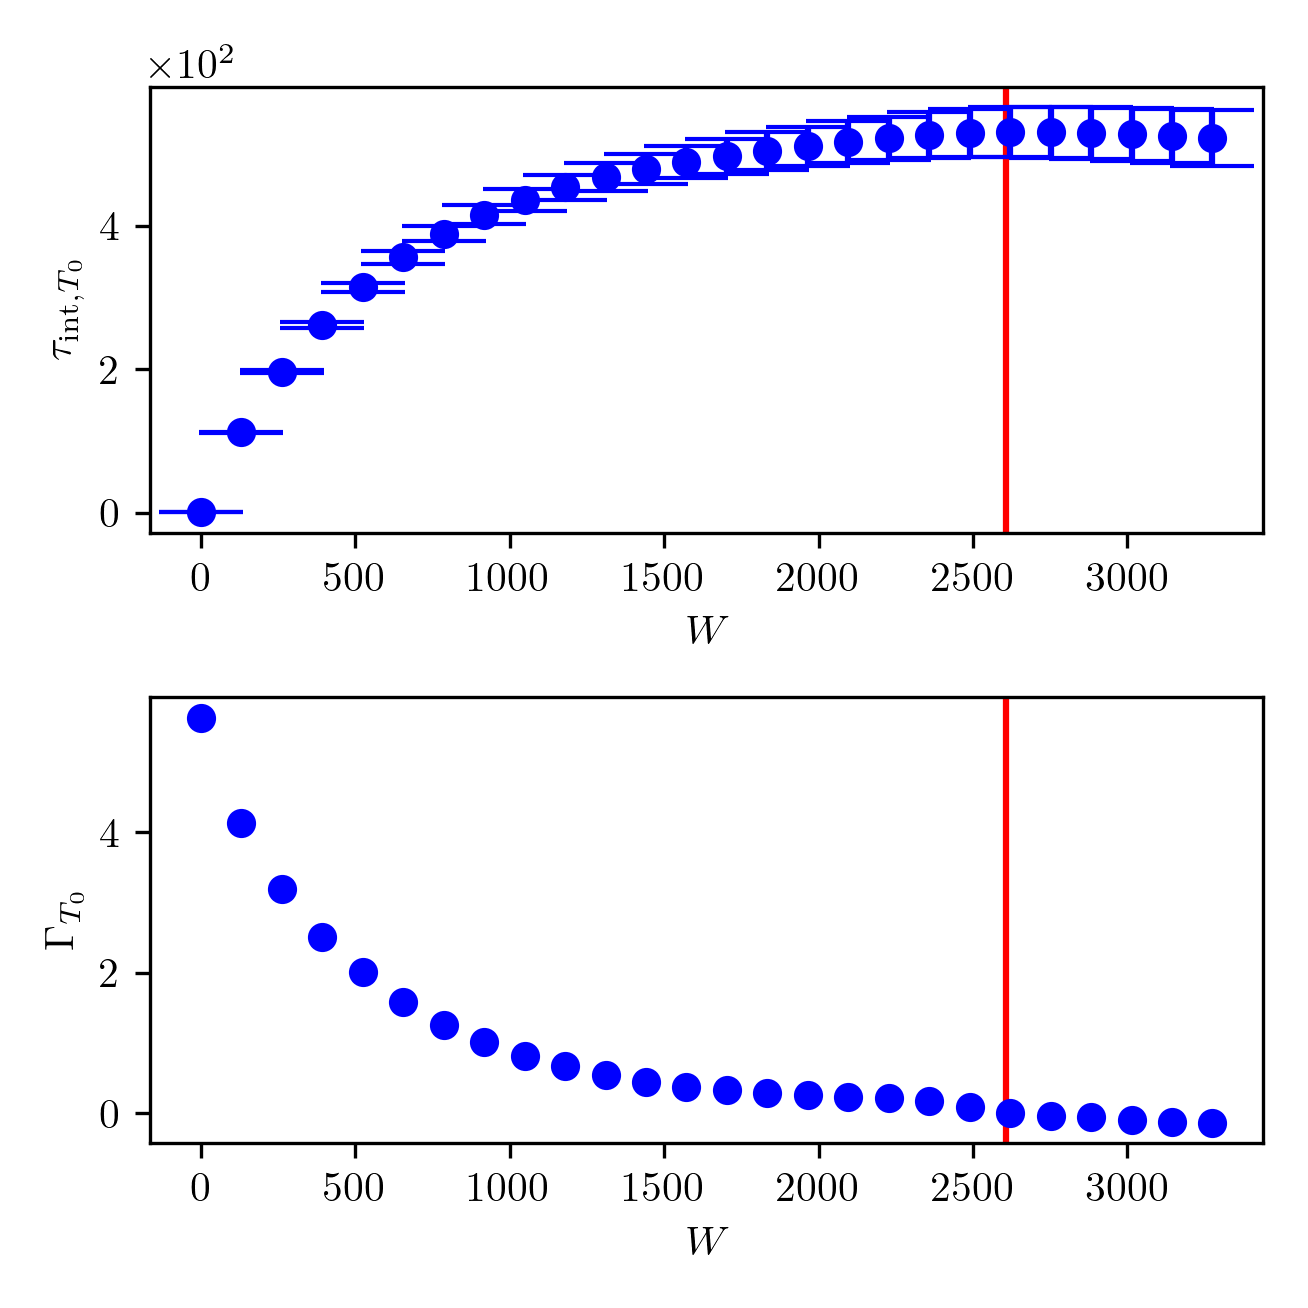
\includegraphics{UwerrTauIntTWalk13.png}
	\caption[IACT and autocorrelation function of samples $a_4 \sim \pi(\cdot|\bm{y})$, for approximated model.]{The IACT $\tau_{\text{int},a_4}$ at summation windows W and the estimated autocorrelation function $\Gamma_{a_4}$ at lag $t$ of samples $a_4 \sim \pi( \cdot| \bm{y})$ from the t-walk for the approximated forward model.
	The estimated IACTs are twice the values provided by~\cite{drikHesse, UwerrM}.}
	\label{fig:TWalkIATC14}
\end{figure}
\begin{figure}[ht!]
	\centering
	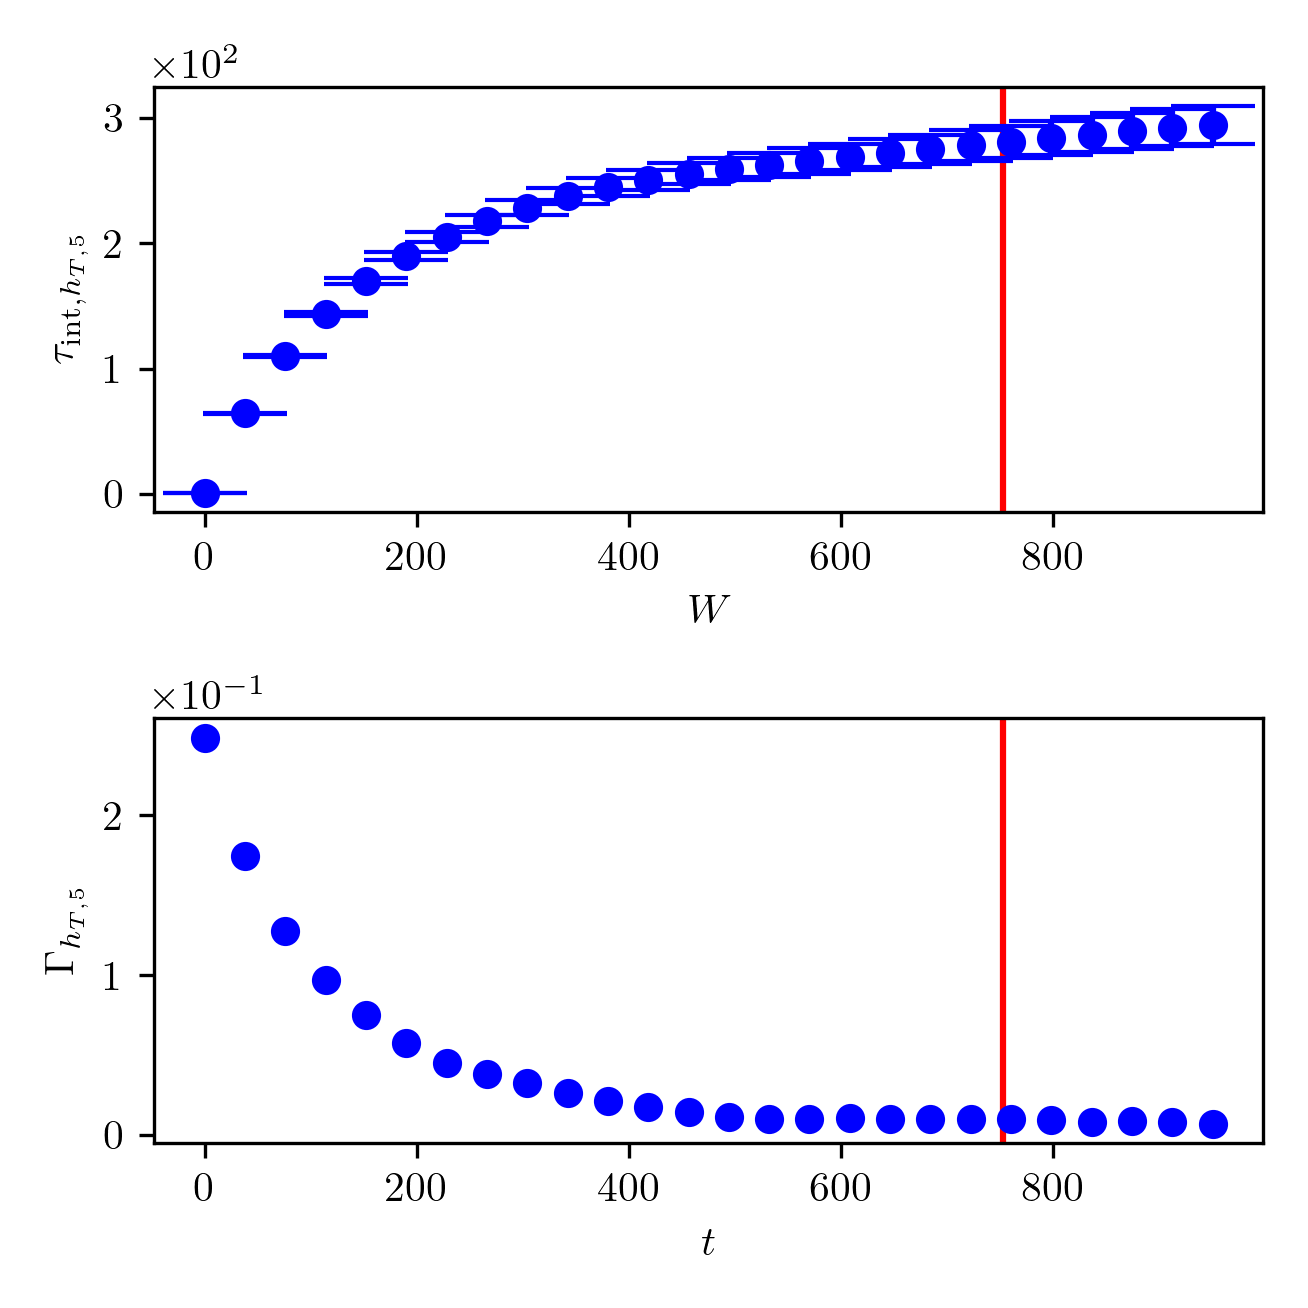
\includegraphics{UwerrTauIntTWalk14.png}
	\caption[IACT and autocorrelation function of samples $h_{T,5} \sim \pi(\cdot|\bm{y})$, for approximated model.]{The IACT $\tau_{\text{int},h_{T,5}}$ at summation windows W and the estimated autocorrelation function $\Gamma_{h_{T,5}}$ at lag $t$ of samples $h_{T,5} \sim \pi( \cdot| \bm{y})$ from the t-walk for the approximated forward model.
	The estimated IACTs are twice the values provided by~\cite{drikHesse, UwerrM}.}
	\label{fig:TWalkIATC15}
\end{figure}

\begin{figure}[ht!]
	\centering
	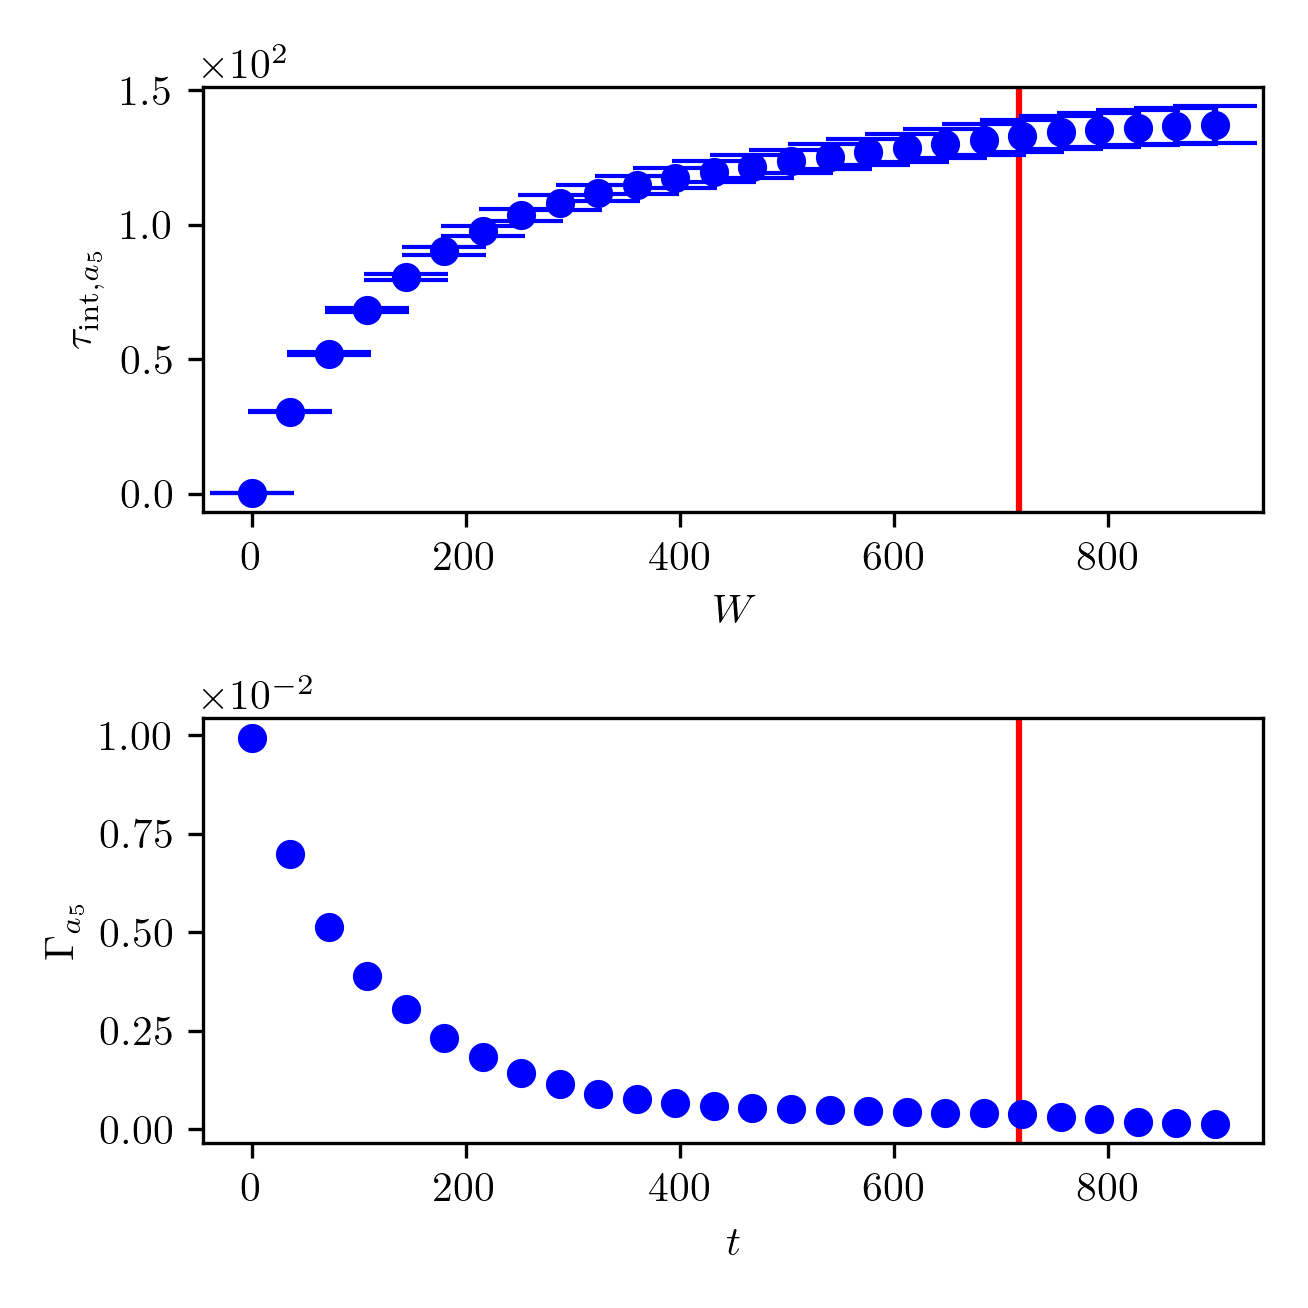
\includegraphics{UwerrTauIntTWalk15.png}
	\caption[IACT and autocorrelation function of samples $a_5 \sim \pi(\cdot|\bm{y})$, for approximated model.]{The IACT $\tau_{\text{int},a_5}$ at summation windows W and the estimated autocorrelation function $\Gamma_{a_5}$ at lag $t$ of samples $a_5 \sim \pi(\cdot| \bm{y})$ from the t-walk for the approximated forward model.
	The estimated IACTs are twice the values provided by~\cite{drikHesse, UwerrM}.}
	\label{fig:TWalkIATC16}
\end{figure}
\begin{figure}[ht!]
	\centering
	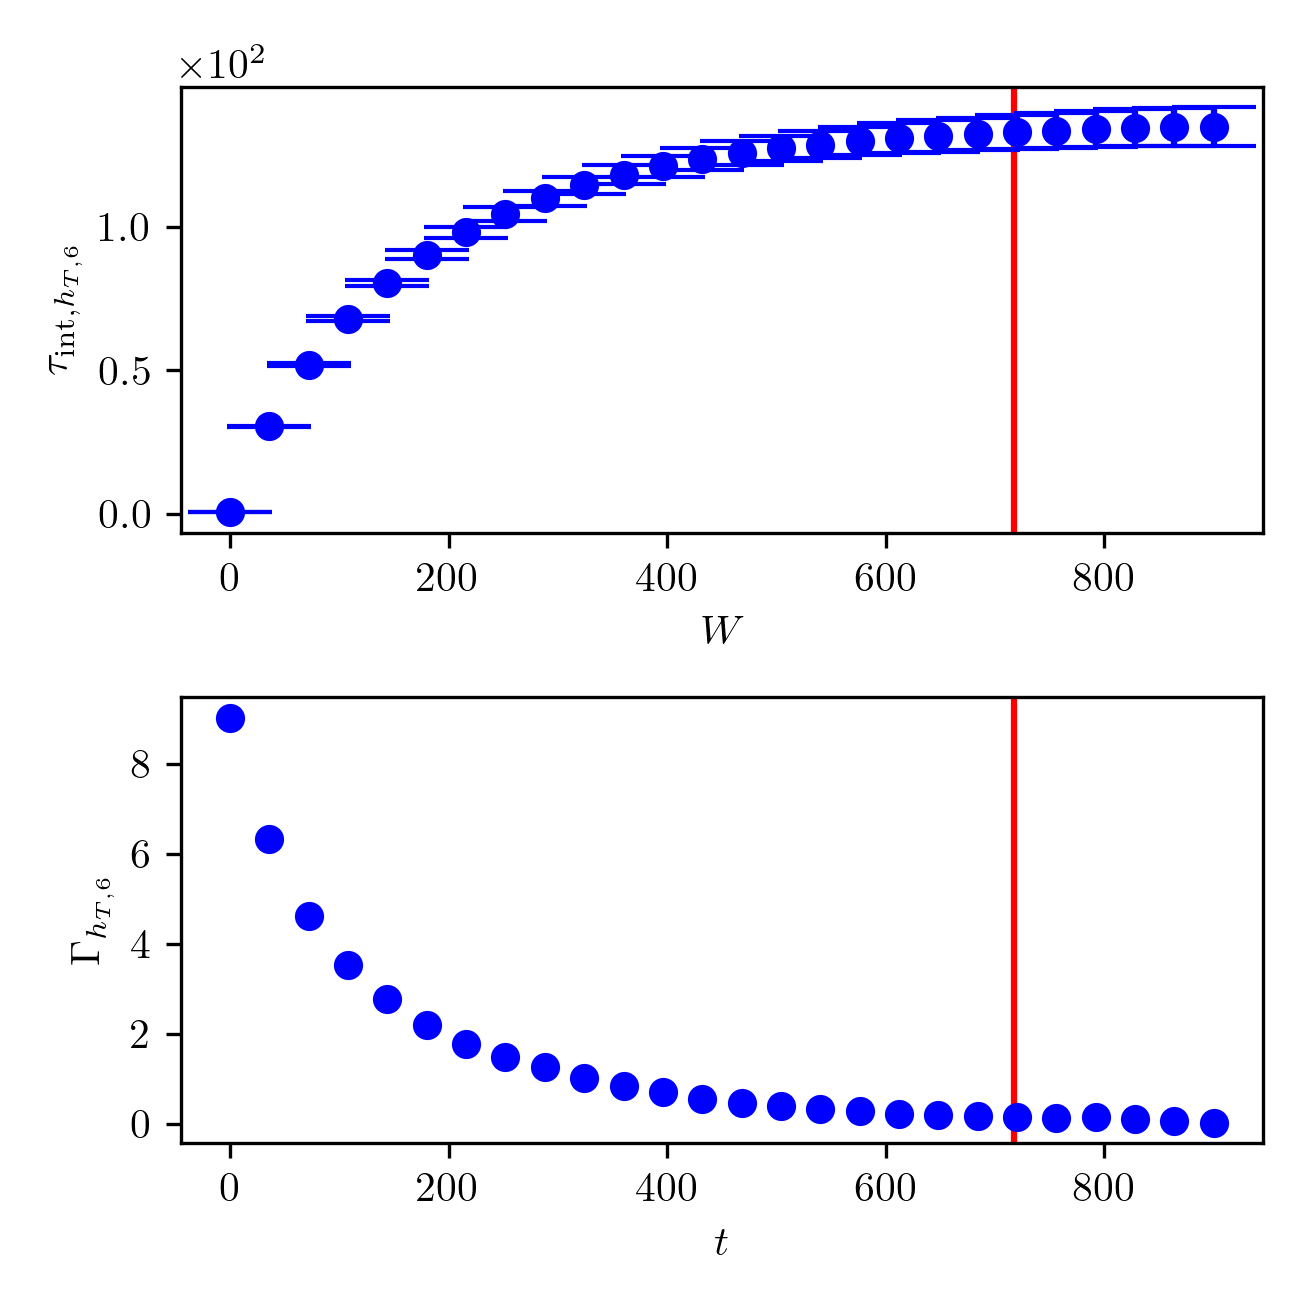
\includegraphics{UwerrTauIntTWalk16.png}
	\caption[IACT and autocorrelation function of samples $h_{T,6} \sim \pi(\cdot|\bm{y})$, for approximated model.]{The IACT $\tau_{\text{int},h_{T,6}}$ at summation windows W and the estimated autocorrelation function $\Gamma_{h_{T,6}}$ at lag $t$ of samples $h_{T,6} \sim \pi( \cdot| \bm{y})$ from the t-walk for the approximated forward model.
	The estimated IACTs are twice the values provided by~\cite{drikHesse, UwerrM}.}
	\label{fig:TWalkIATC17}
\end{figure}

\begin{figure}[ht!]
	\centering
	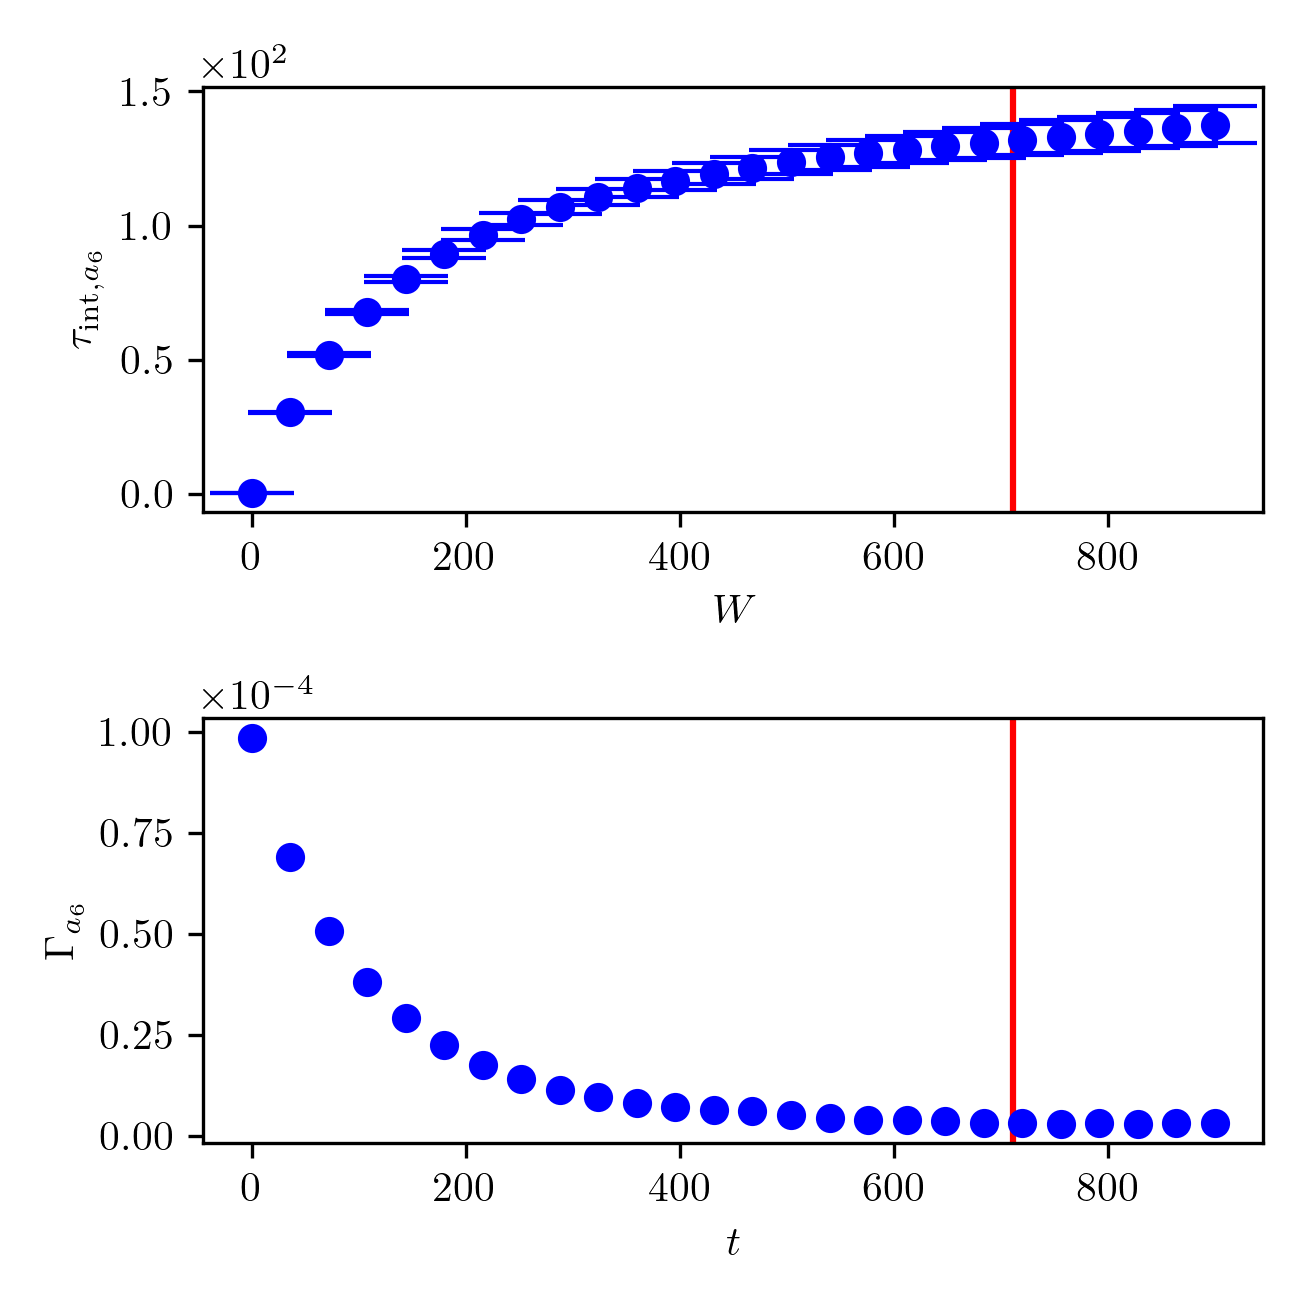
\includegraphics{UwerrTauIntTWalk17.png}
	\caption[IACT and autocorrelation function of samples $a_6 \sim \pi(\cdot|\bm{y})$, for approximated model.]{The IACT $\tau_{\text{int},a_6}$ at summation windows W and the estimated autocorrelation function $\Gamma_{a_6}$ at lag $t$ of samples $a_6 \sim \pi( \cdot| \bm{y})$ from the t-walk for the approximated forward model.
	The estimated IACTs are twice the values provided by~\cite{drikHesse, UwerrM}.}
	\label{fig:TWalkIATC18}
\end{figure}





